\capitulo{5}{Resultados}
En esta sección se presentan los resultados obtenidos mediante la simulación de los modelos SI, SIS, SIR y SEIR, tanto en sus versiones básicas como con vacunación, utilizando Simulink. 

Es importante destacar que el parámetro $\beta$ que se emplea en los modelos corresponde a la tasa de transmisión ajustada o efectiva, aque para simplificar a partir de ahora se denominará solo beta, aunque sea la efectiva.

\section{Comportamiento modelo SI}
Para el modelo SI se han realizado tres simulaciones con distintos valores de $\beta$ y condiciones iniciales, tal como se resume en la Tabla \ref{tab:resultadosSI}. Estas simulaciones permiten analizar cómo varía la propagación de una infección.
\begin{table}[H]
\centering
\begin{tabular}{|c|c|c|c|}
\hline
\textbf{Parámetro} & \textbf{Suimulación 1} & \textbf{Simulación 2} & \textbf{Simulación 3} \\
\hline
Susceptibles (S) & 999 & 9990 & 9990 \\
\hline
Infectados (I)  & 1 & 10   & 10   \\
\hline
\(\beta\)   & 0.00005     & 0.000001 & 0.000008 \\
\hline
\end{tabular}
\caption{Datos usados para ver el comportamiento del modelo SI.}
\label{tab:resultadosSI}
\end{table}
A continuación, se presentan los resultados de cada simulación en las figuras (\ref{fig:simulación 1 SI})(\ref{fig:simulacion 2 SI})(\ref{fig:simulacion 3 SI}). 
\begin{figure}[H]
    \centering
    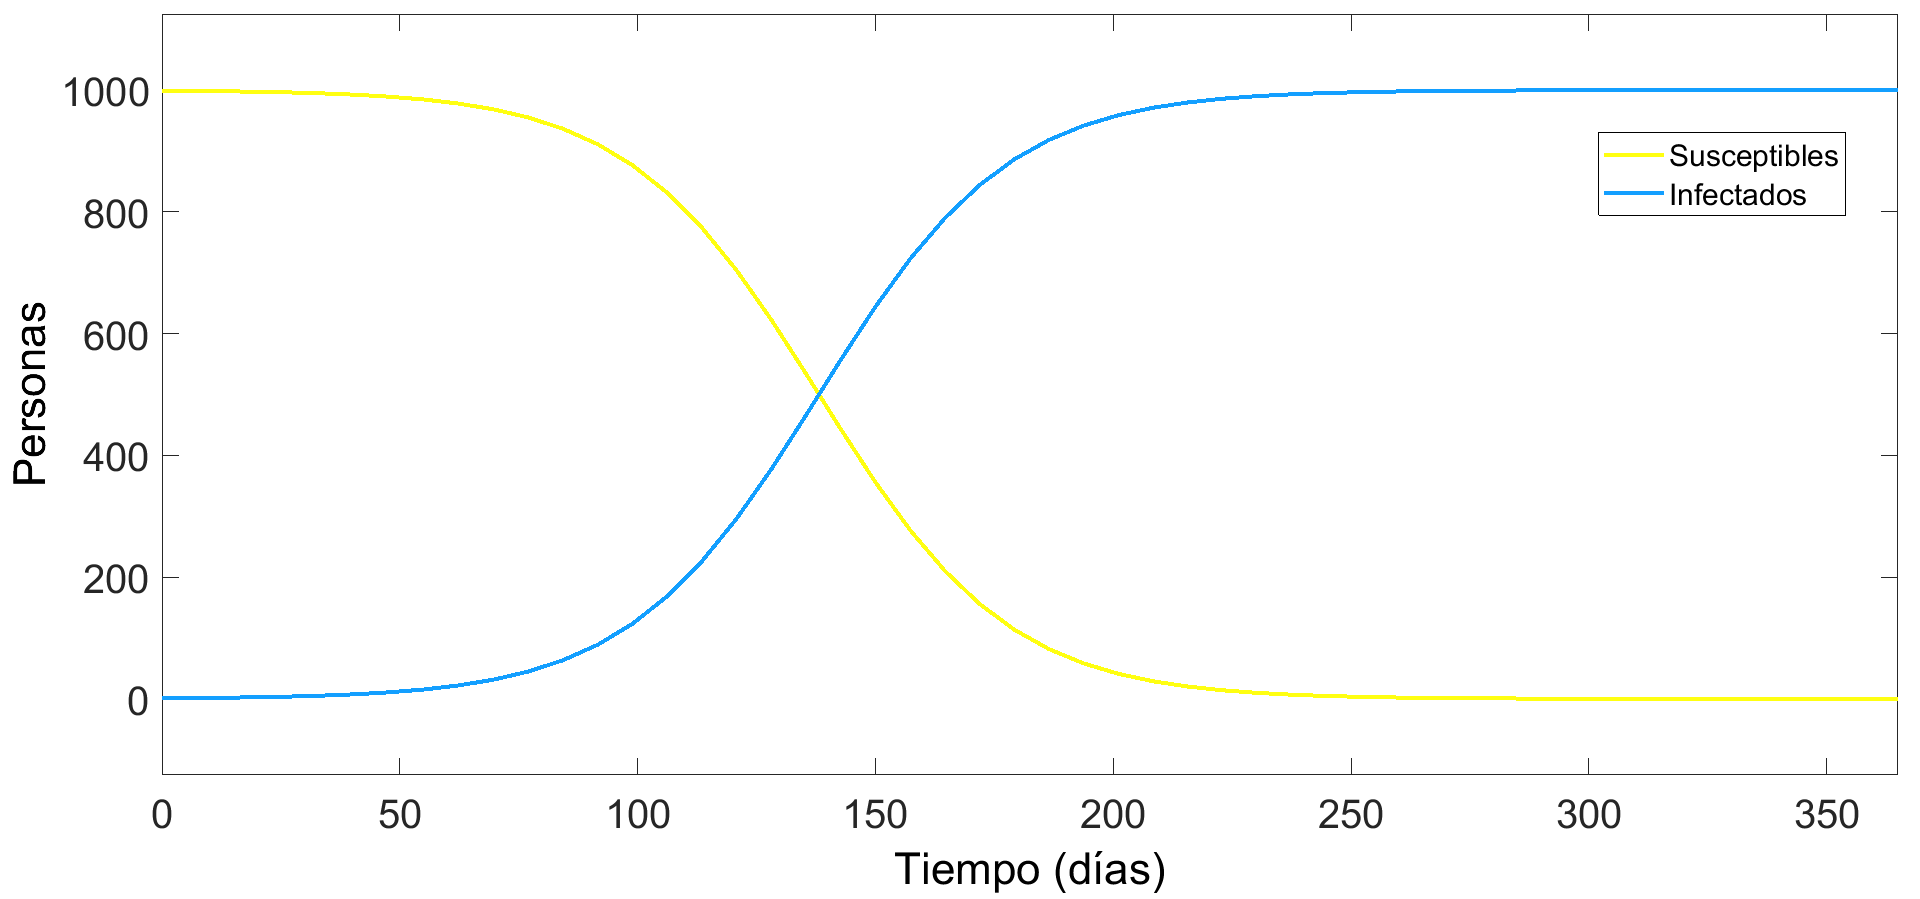
\includegraphics[width=0.7\textwidth]{img/modelo_SI_resultado_ejemplo.png}
    \caption{Resultado modelo SI con beta de 0.00005}
    \label{fig:simulación 1 SI}
    \vspace{0.5cm} % Ajusta el espacio vertical entre la imagen y el texto
\end{figure}

\begin{figure}[H]
    \centering
    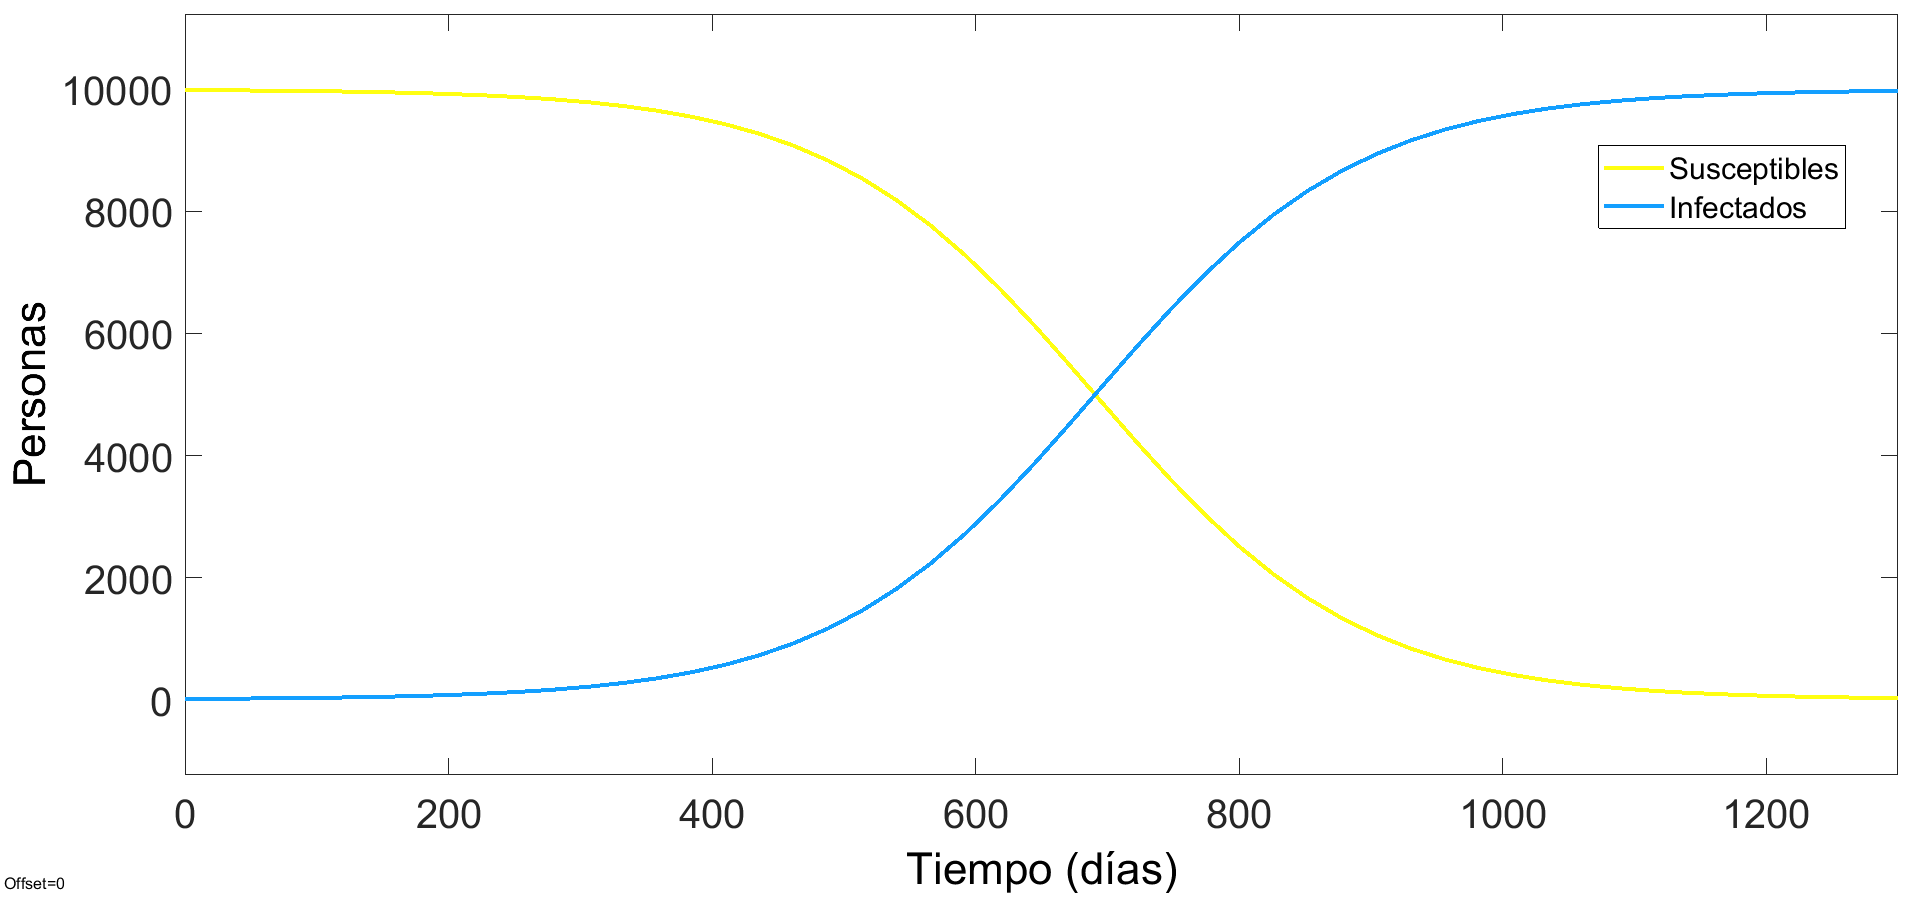
\includegraphics[width=0.7\textwidth]{img/modelo_SI_0.1.png}
    \caption{Resultado modelo SI con beta de 0.000001}
    \label{fig:simulacion 2 SI}
    \vspace{0.5cm} % Ajusta el espacio vertical entre la imagen y el texto
\end{figure}

\begin{figure}[H]
    \centering
    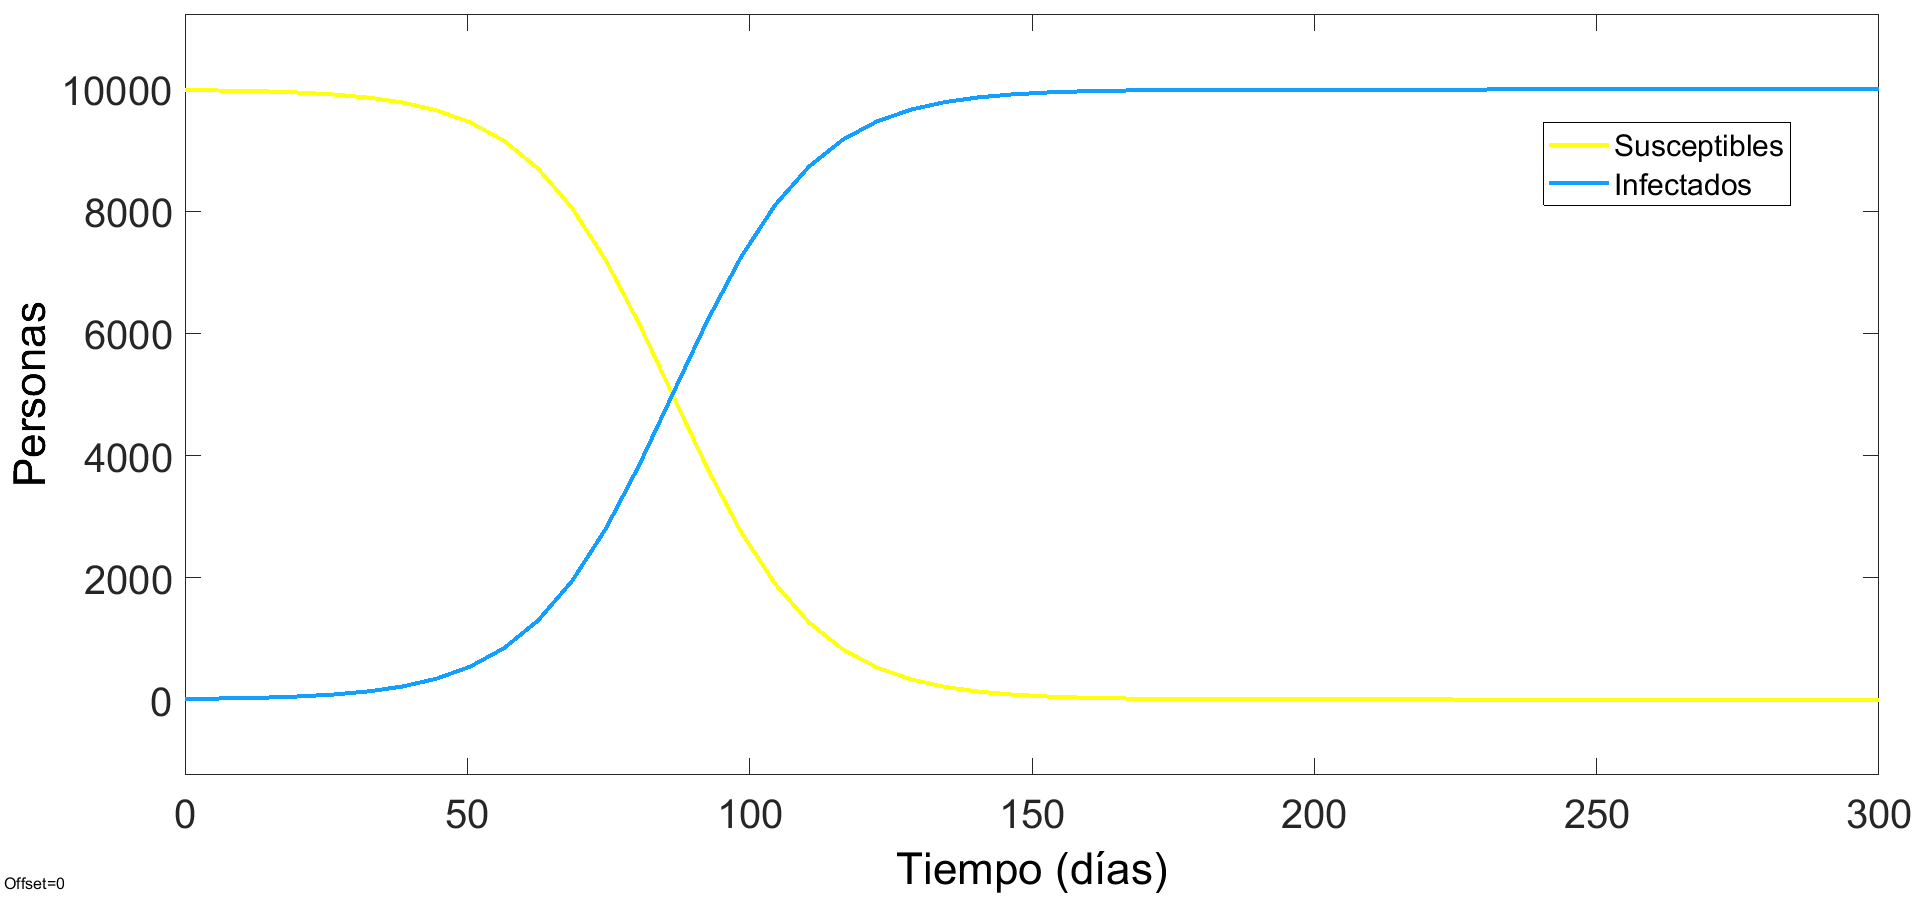
\includegraphics[width=0.7\textwidth]{img/modelo_SI_08.png}
    \caption{Resultado modelo SI con beta de 0.000008}
    \label{fig:simulacion 3 SI}
    \vspace{0.5cm} % Ajusta el espacio vertical entre la imagen y el texto
\end{figure}

Como se puede observar en las simulaciones, independientemente del valor de $\beta$, todos los individuos susceptibles acaban infectándose con el paso del tiempo. La tasa de transmisión únicamente influye en la velocidad a la que se propaga la infección, pero no en el resultado final. Esto es coherente con el comportamiento esperado del modelo SI, en el que no existe recuperación ni inmunidad, lo que implica que el número de infectados tiende a igualar la población total a largo plazo.


\subsection{Comportamiento epidemia SIDA/VIH}
A continuación, se presenta la simulación del comportamiento de la epidemia del VIH/SIDA, utilizando los parámetros definidos anteriormente en el apartado de descripción de los datos. La figura \ref{fig:vih} muestra la evolución de la enfermedad a lo largo del tiempo, destacando cómo se comporta la dinámica de contagio bajo el modelo utilizado.

\begin{figure}[H]
    \centering
    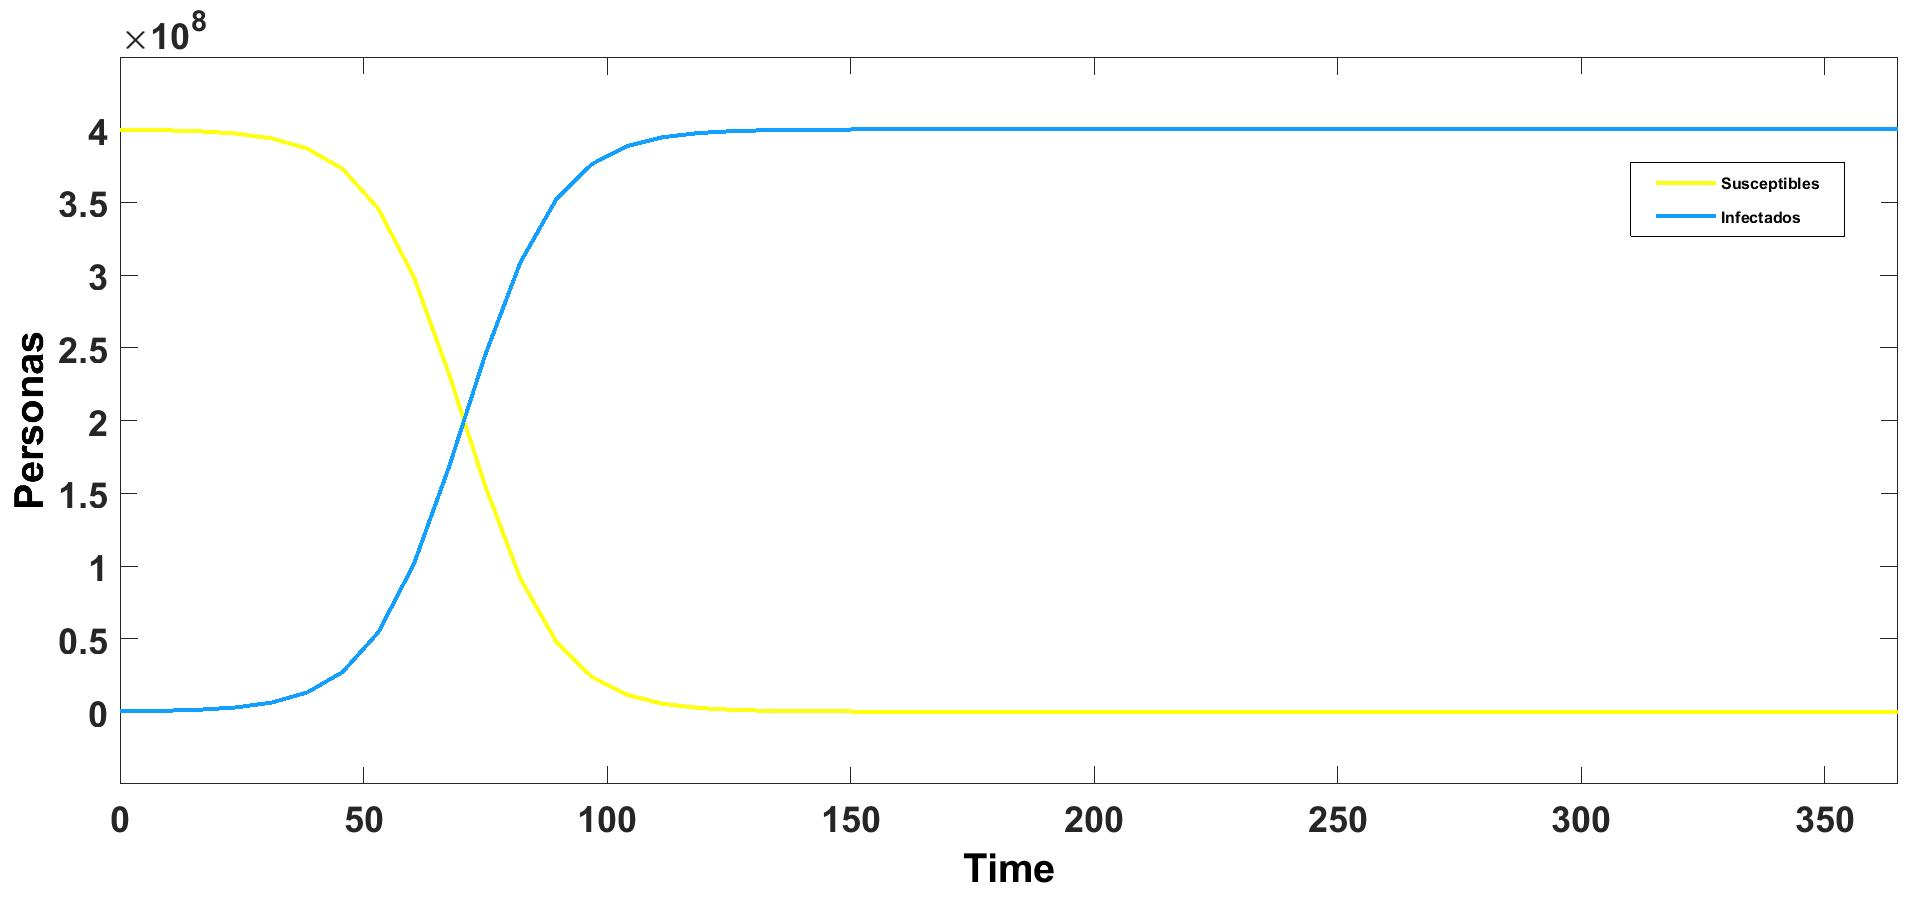
\includegraphics[width=0.7\textwidth]{img/modelo_SI.jpg}
    \caption{Resultado modelo SI con los datos reales para el VIH/SIDA}
    \label{fig:vih}
    \vspace{0.5cm} % Ajusta el espacio vertical entre la imagen y el texto
\end{figure}

Tras simularlo la grafica \ref{fig:vih} muestra la evolución de la enfermedad en la región MENA a lo largo de un periodo de 365 días, 1 año, utilizando el modelo SI con los parámetros definidos previamente.
La línea amarilla representa el número de personas susceptibles, las que no han contraído la enfermedad, mientras que a línea azul muestra el número de personas infectadas, aquellas que han adquirido la enfermedad y permanecen en este estado, no hay recuperación.
Al principio de la simulación, casi toda la población es susceptible (400 millones de personas) y solo una pequeña fracción se encuentra infectada (240mil personas). Sin embargo, debido a la tasa de transmisión $\beta$ ajustada, se observa un crecimiento exponencial del número de infectados.
Hacia el día 70, la curva de infectados y la de susceptibles se cruzan: a partir de este punto, la mayoría de la población ya está infectada. Finalmente, tras aproximadamente 100 días, la curva de personas infectadas se estabiliza cerca del total de la población, mientras que la de susceptibles tiende a cero.



\section{Comportamiento modelo SIS}
Para el modelo SIS se han realizado simulaciones con distintos
valores para los parámetros como para las condiciones iniciales. Los datos utilizados se representan en la tabla \ref{tab:datos para modelo SIS}
\begin{table}[H]
\centering
\begin{tabular}{|c|c|c|c|}
\hline
\textbf{Parámetro} & \textbf{Simulación 1} & \textbf{Simulación 2}  & \textbf{Simulación 3}\\
\hline
Susceptibles (S) & 990 & 8000 & 9990\\
\hline
Infectados (I)   & 10   & 2000 & 10  \\
\hline
\(\beta\)        & 0.001 & 0.0002  & 0.0007\\
\hline
\(\gamma\)        & 0.08 & 0.3 & 0.15\\
\hline
\end{tabular}
\caption{Datos usados para ver el comportamiento del modelo SIS.}
\label{tab:datos para modelo SIS}
\end{table}

Se presentan los resultados de cada simulación en las figuras (\ref{fig:simulacion 1 SIS})(\ref{fig:simulación 2 SIS})(\ref{fig:Simulación 3 SIS})

\begin{figure}[H]
    \centering
    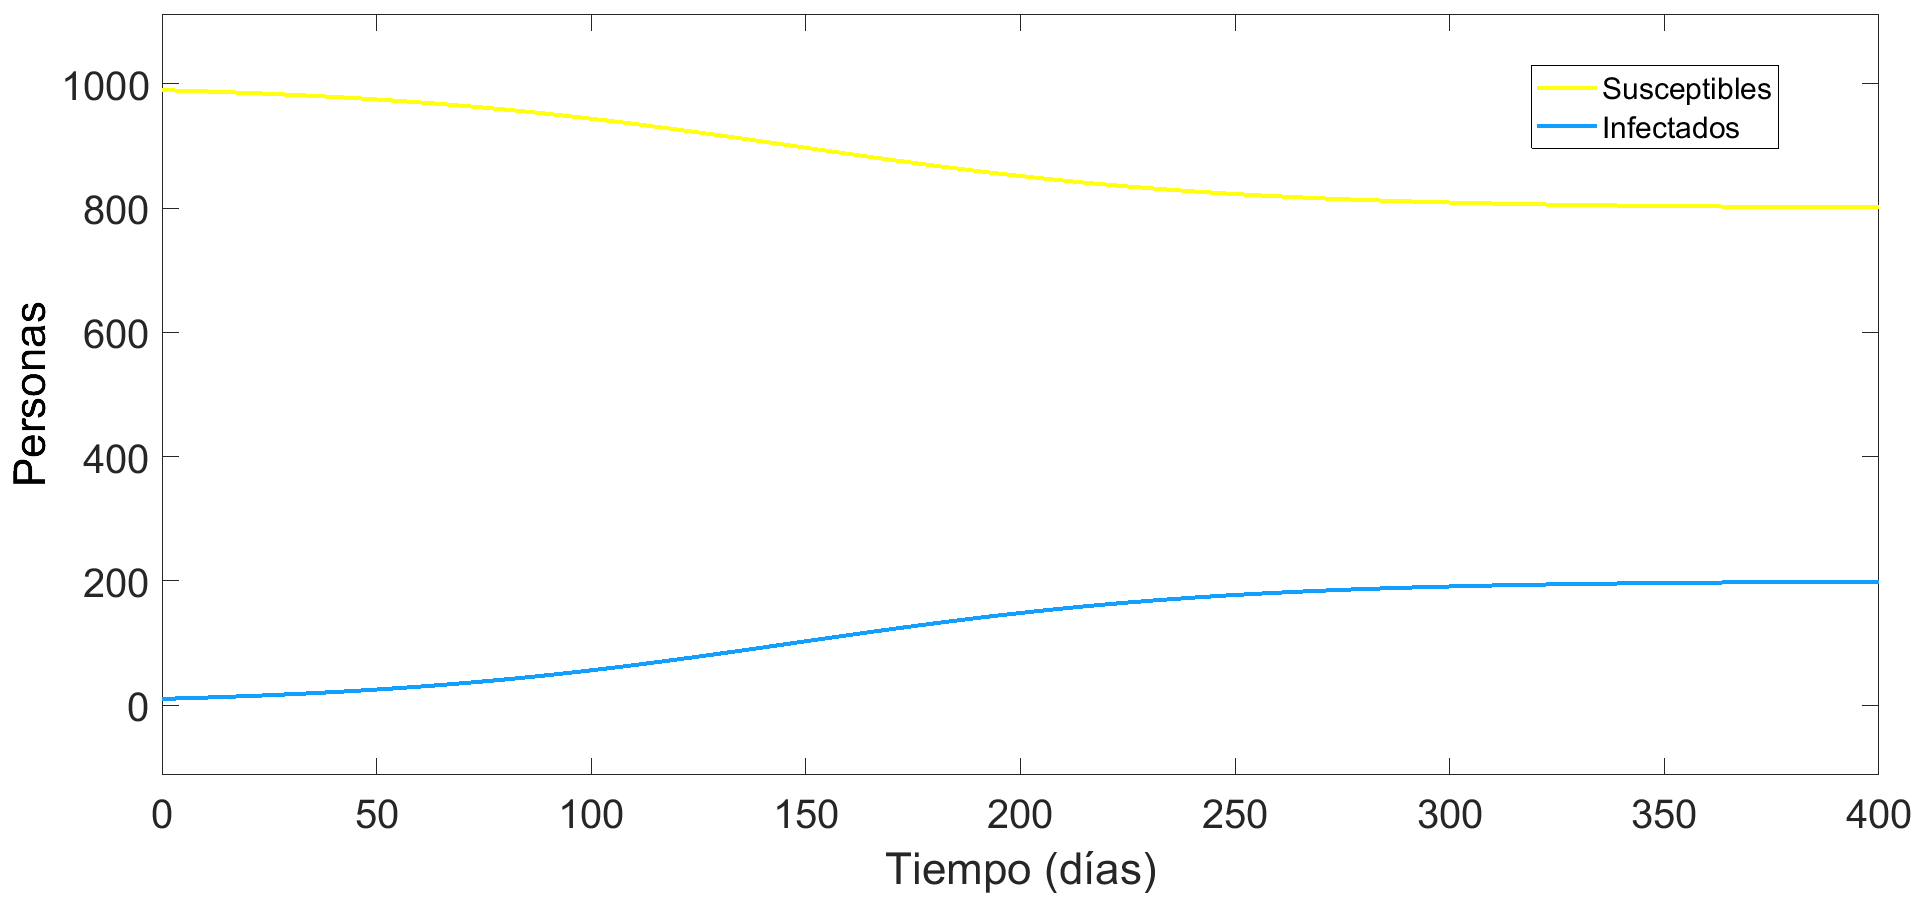
\includegraphics[width=0.7\textwidth]{img/modelo_SIS_1_08.png}
    \caption{Resultado modelo SIS con beta 0.001 y gamma 0.08}
    \label{fig:simulacion 1 SIS}
    \vspace{0.5cm} % Ajusta el espacio vertical entre la imagen y el texto
\end{figure}

\begin{figure}[H]
    \centering
    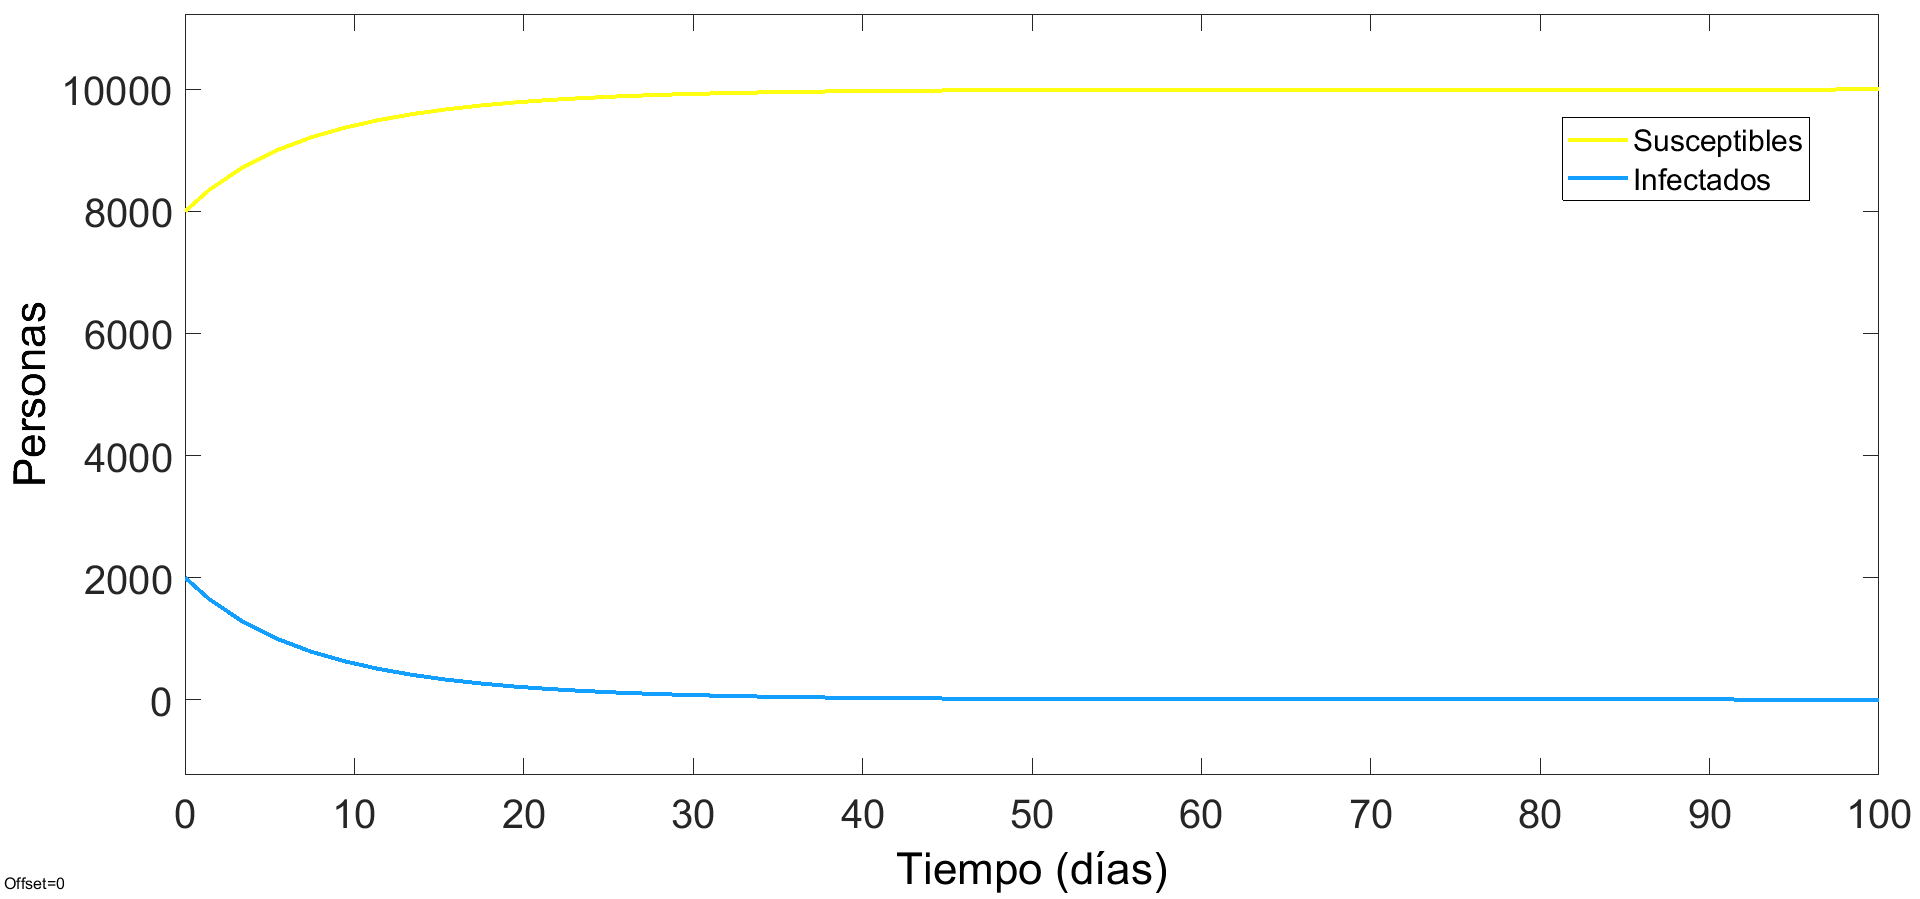
\includegraphics[width=0.7\textwidth]{img/modelo_SIS_2_3.png}
    \caption{Resultado modelo SIS con beta 0.0002 y gamma 0.3}
    \label{fig:simulación 2 SIS}
    \vspace{0.5cm} % Ajusta el espacio vertical entre la imagen y el texto
\end{figure}

\begin{figure}[H]
    \centering
    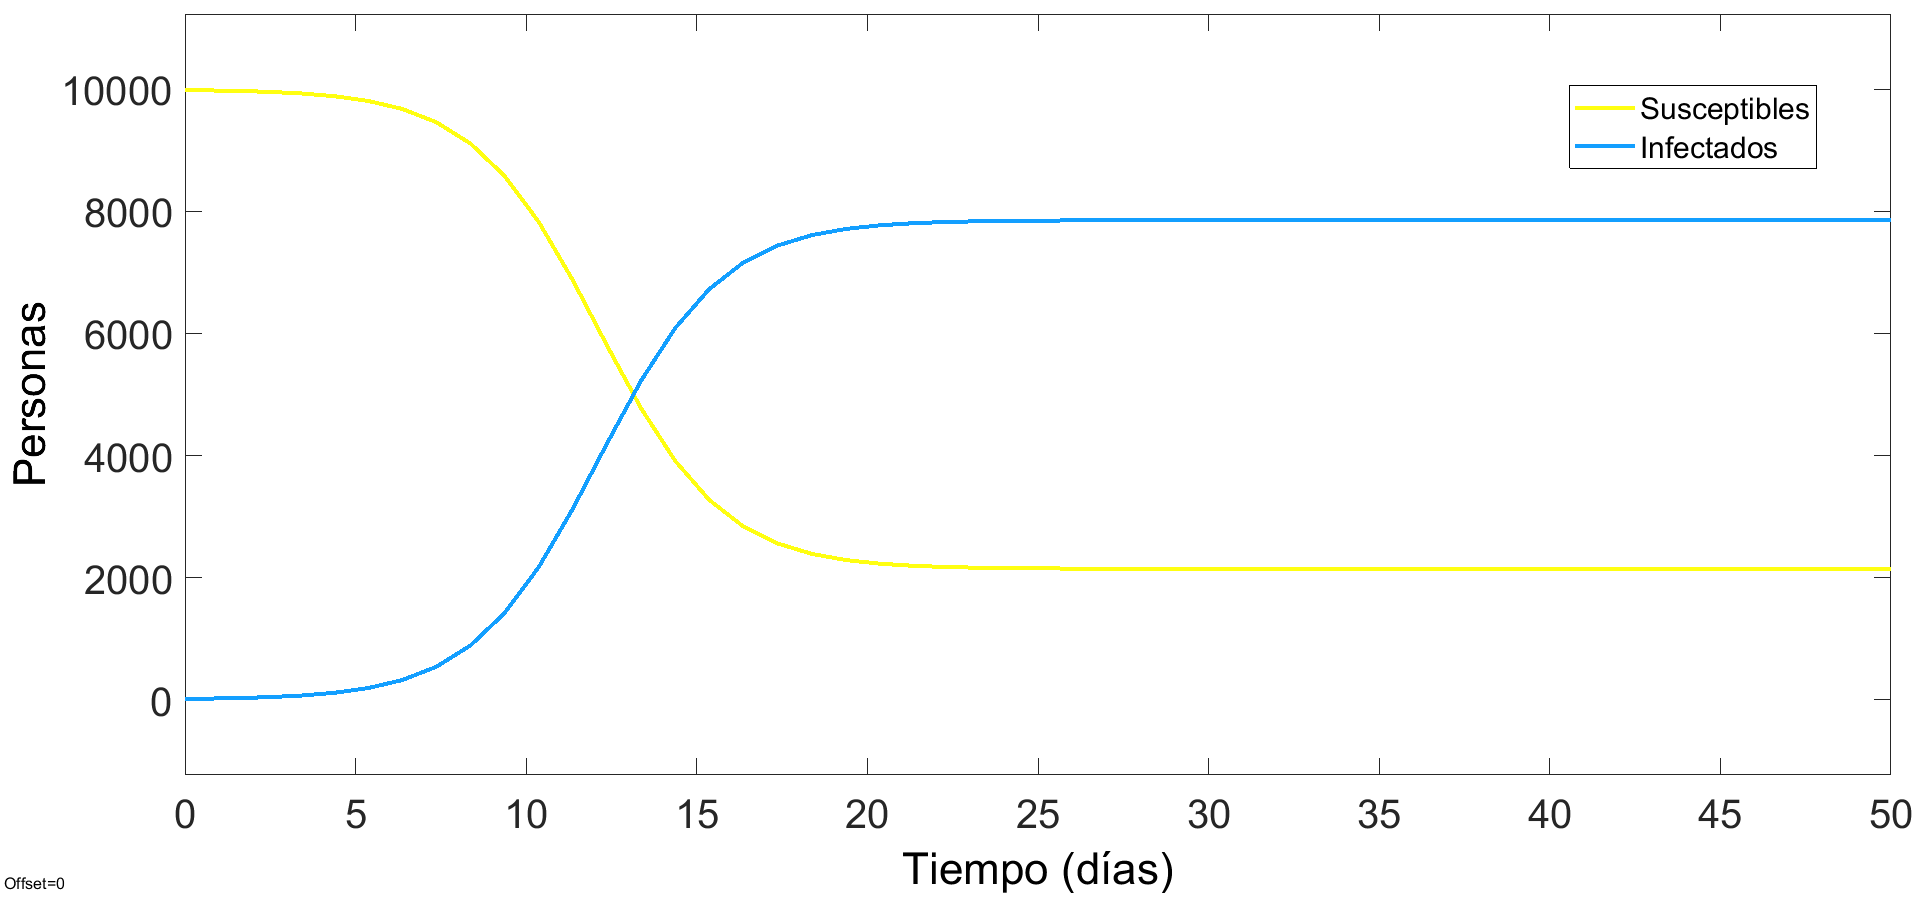
\includegraphics[width=0.7\textwidth]{img/modelo_SIS_7_15.png}
    \caption{Resultado modelo SIS con beta 0.0007 y gamma 0.15}
    \label{fig:Simulación 3 SIS}
    \vspace{0.5cm} % Ajusta el espacio vertical entre la imagen y el texto
\end{figure}

Para la figura \ref{fig:simulacion 1 SIS} se ve que los infectados aumentan ligeramente en un principio y se estabilizan en un valor muy bajo, mientras que los susceptibles pasa lo contrario. La enfermedad se mantiene endémica con proporción baja de infectados, alcanzando un equilibrio.
Para la figura \ref{fig:simulación 2 SIS} los infectados disminuyen rápido hasta desaparecer, mientras que los infectados auumentan hasta llegar a ser todos de nuevo susceptibles. Se evoluciona hacia un estado libre de infección. Eliminación de la enfermedad y recuperación de la población susceptible. Por último, en la figura \ref{fig:Simulación 3 SIS} la enfermedad no desaparece, sino que se mantiene permanente en la población, en este caso con más personas infectadas que susceptibles. El modelo acaba en un equilibrio, donde los contagios y las recuperaciones se equilibran. Los infectados no desaparecen y no se contagia toda la población ya que existe la recuperación. Se convierte en una enfermedad endémica, permanece estable en la población

\subsection{Comportamiento epidemia gonorrea}
A continuación, se presenta  la simulación del comportamiento de la epidemia de la gonorrea, utilizando los parámetros definidos anteriormente en el apartado de descripción de los datos. La figura \ref{fig:simugono} muestra la evolución de la enfermedad a lo largodel tiempo, destacando la dinámica de contagio bajo el modelo utilizado.

\begin{figure}[H]
    \centering
    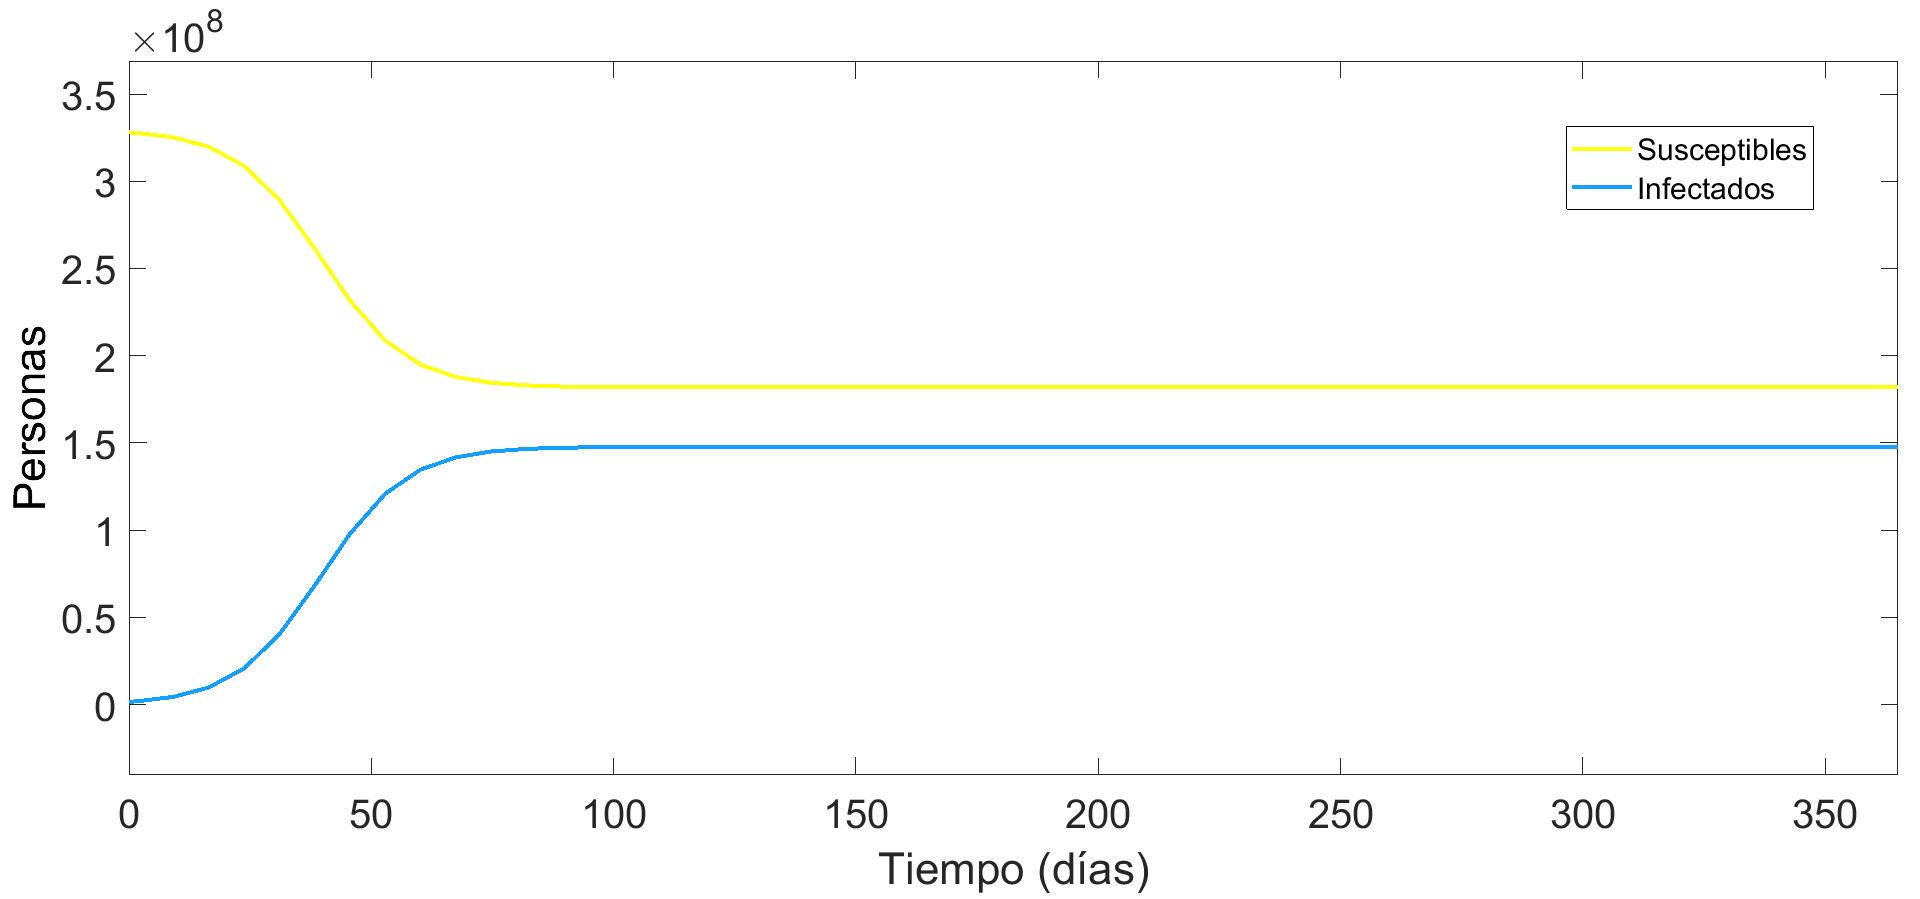
\includegraphics[width=0.7\textwidth]{img/modelo_SIS.jpg}
    \caption{Resultado modelo SIS con los datos reales para la gonorrea}
    \label{fig:simugono}
    \vspace{0.5cm} % Ajusta el espacio vertical entre la imagen y el texto
\end{figure}

La gráfica obtenida \ref{fig:simugono} tras simular el modelo SIS muestra la evolución temporal de la infección a lo largo de un año. Se observa que inicialmente el número de infectados crece de forma acelerada, mientras que la cantidad de individuos susceptibles disminuye de manera brusca. Esta fase inicial refleja el momento en el que la transmisión domina sobre la recuperación, debido a la elevada proporción de individuos susceptibles y la presencia activa de personas infectadas.
Conforme transcurren los días, la velocidad de crecimiento de la infección disminuye y ambas curvas comienzan a estabilizarse. Esto indica que el sistema alcanza un equilibrio epidemiológico estable, característico del modelo SIS, en el que el número de nuevas infecciones diarias se compensa con el número de recuperaciones. Dado que los individuos recuperados no adquieren inmunidad y vuelven al compartimento de susceptibles, la enfermedad no desaparece, sino que persiste con una proporción constante de la población infectada.
Se calcula el número básico de reproducción en la ecuación \eqref{eq:R0_179}.
\begin{equation}
R_0 = \frac{\beta}{\gamma} = \frac{0.25}{0.14} \approx 1{,}79
\label{eq:R0_179}
\end{equation}
Lo que significa que de media cada persona infectada contagiará aproximadamente a 1,79 personas al día mientras este infectada. Como este valor es mayor que uno, se cumple la condición para que la infección se propague en la población y no desaparezca, como se observa en el resultado de la gráfica. Esto implica que los individuos pueden volver a infectarse. El $R_0$ > 1 indica que la tasa de nuevas infecciones supera a la tasa de recuperaciones, y que la enfermedad se propagará hasta que se alcance un equilibrio endémico. En este equilibrio, la proporción de personas infectadas y susceptibles se mantiene constante en el tiempo.





\section{Comportamiento modelo SIR}
Para el modelo SIR se han realizado varias simulaciones con valores distintos para las condiciones iniciales y parámetros. Los datos que se utilizan se encuentran en la tabla \ref{tab:datos para modelo SIR}.
\begin{table}[H]
\centering
\begin{tabular}{|c|c|c|c|}
\hline
\textbf{Parámetro} & \textbf{Simulación 1} & \textbf{Simulación 2}  & \textbf{Simulación 3}\\
\hline
Susceptibles (S) & 9900 & 8000 & 9900\\
\hline
Infectados (I)   & 100   & 2000 & 100  \\
\hline
Recuperados (R)   &  0   & 0 & 0  \\
\hline
\(\beta\)        & 0.00007 & 0.0002  & 0.0003\\
\hline
\(\gamma\)        & 0.01 & 0.4 & 0.2\\
\hline
\end{tabular}
\caption{Datos usados para ver el comportamiento del modelo SIR}
\label{tab:datos para modelo SIR}
\end{table}

Se observan los resultados para cada simulación en las siguientes figuras (\ref{fig:Simulación 1 SIR})(\ref{fig:Simulación 2 SIR})(\ref{fig:Simulación 3 SIR})

\begin{figure}[H]
    \centering
    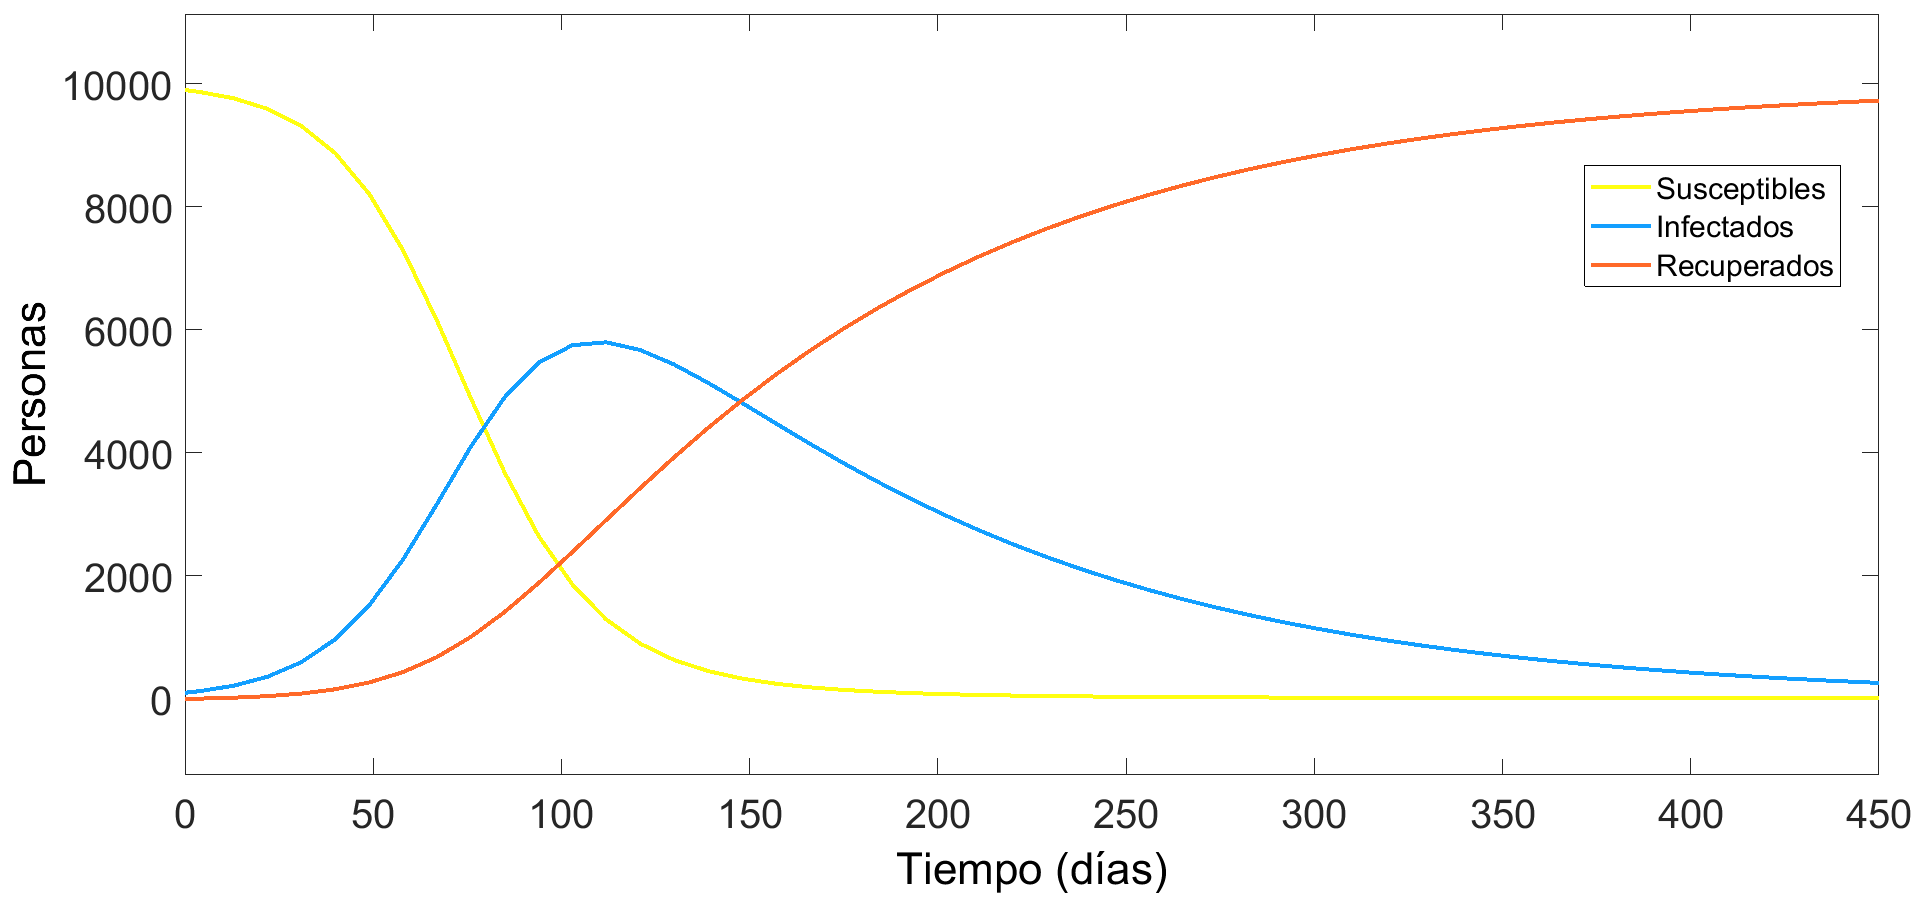
\includegraphics[width=0.7\textwidth]{img/modelo_SIR_0701.png}
    \caption{Resultado modelo SIR con beta 0.000007 y gamma 0.01}
    \label{fig:Simulación 1 SIR}
    \vspace{0.5cm} % Ajusta el espacio vertical entre la imagen y el texto
\end{figure}

\begin{figure}[H]
    \centering
    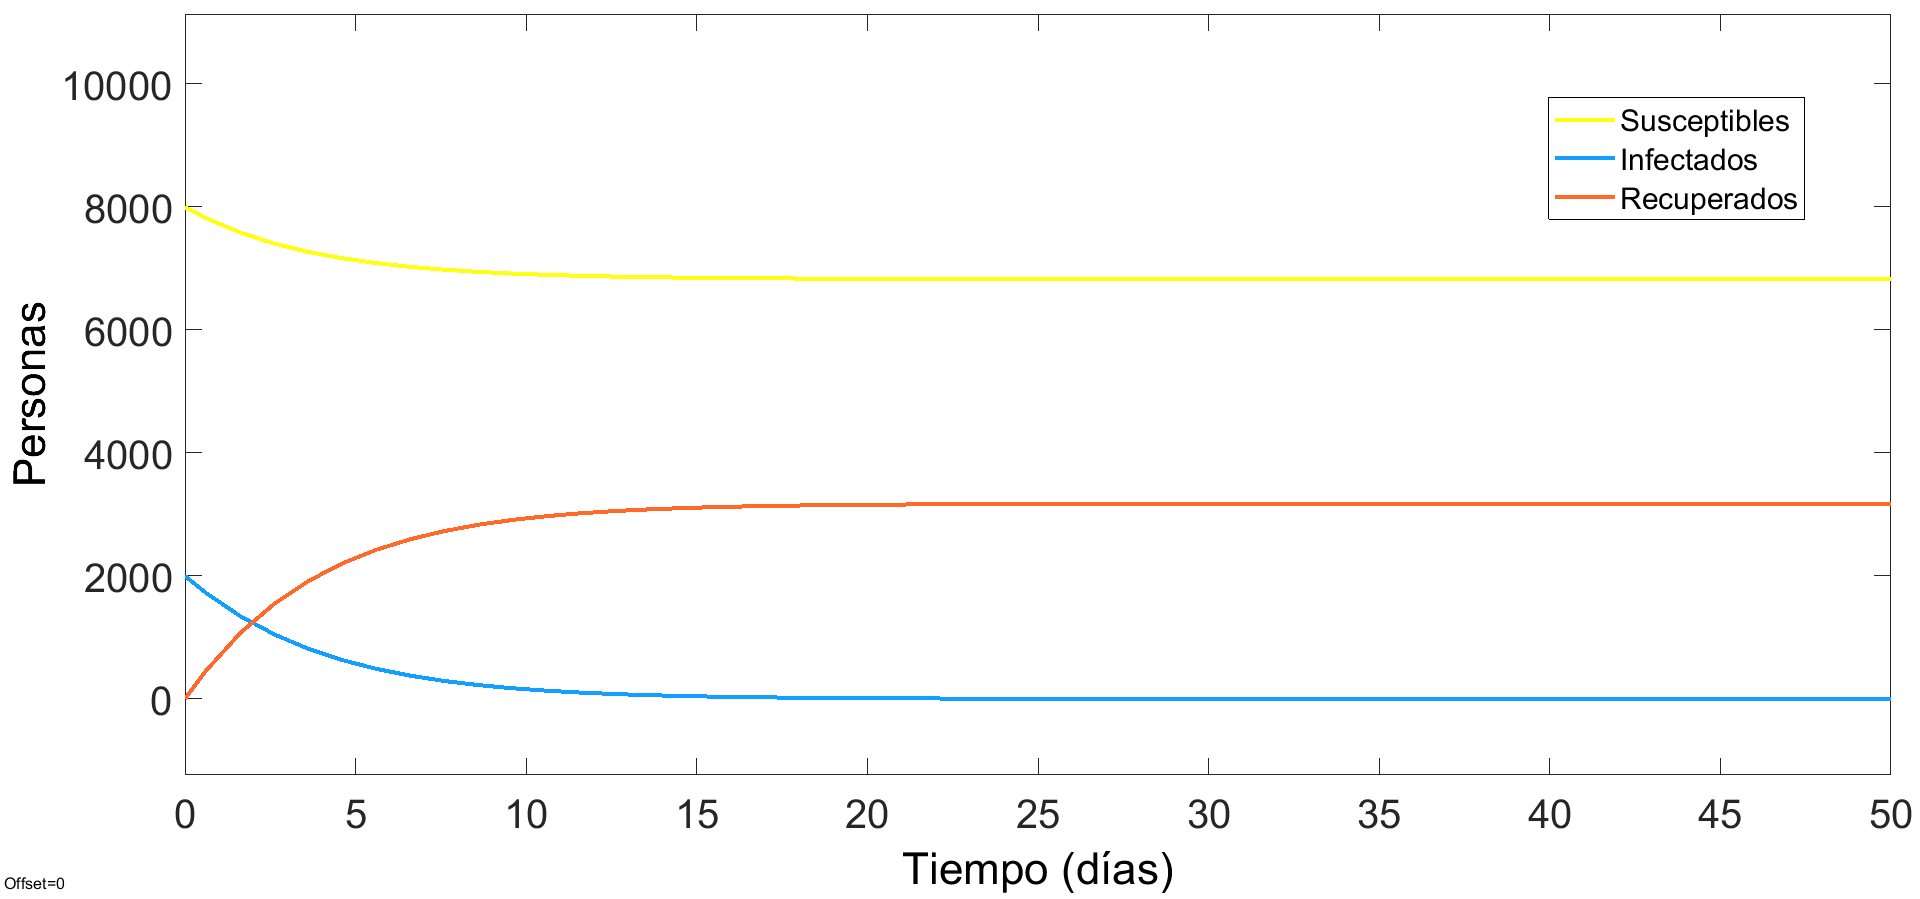
\includegraphics[width=0.7\textwidth]{img/modelo_SIR_24.png}
    \caption{Resultado modelo SIR con beta 0.0002 y gamma 0.4}
    \label{fig:Simulación 2 SIR}
    \vspace{0.5cm} % Ajusta el espacio vertical entre la imagen y el texto
\end{figure}

\begin{figure}[H]
    \centering
    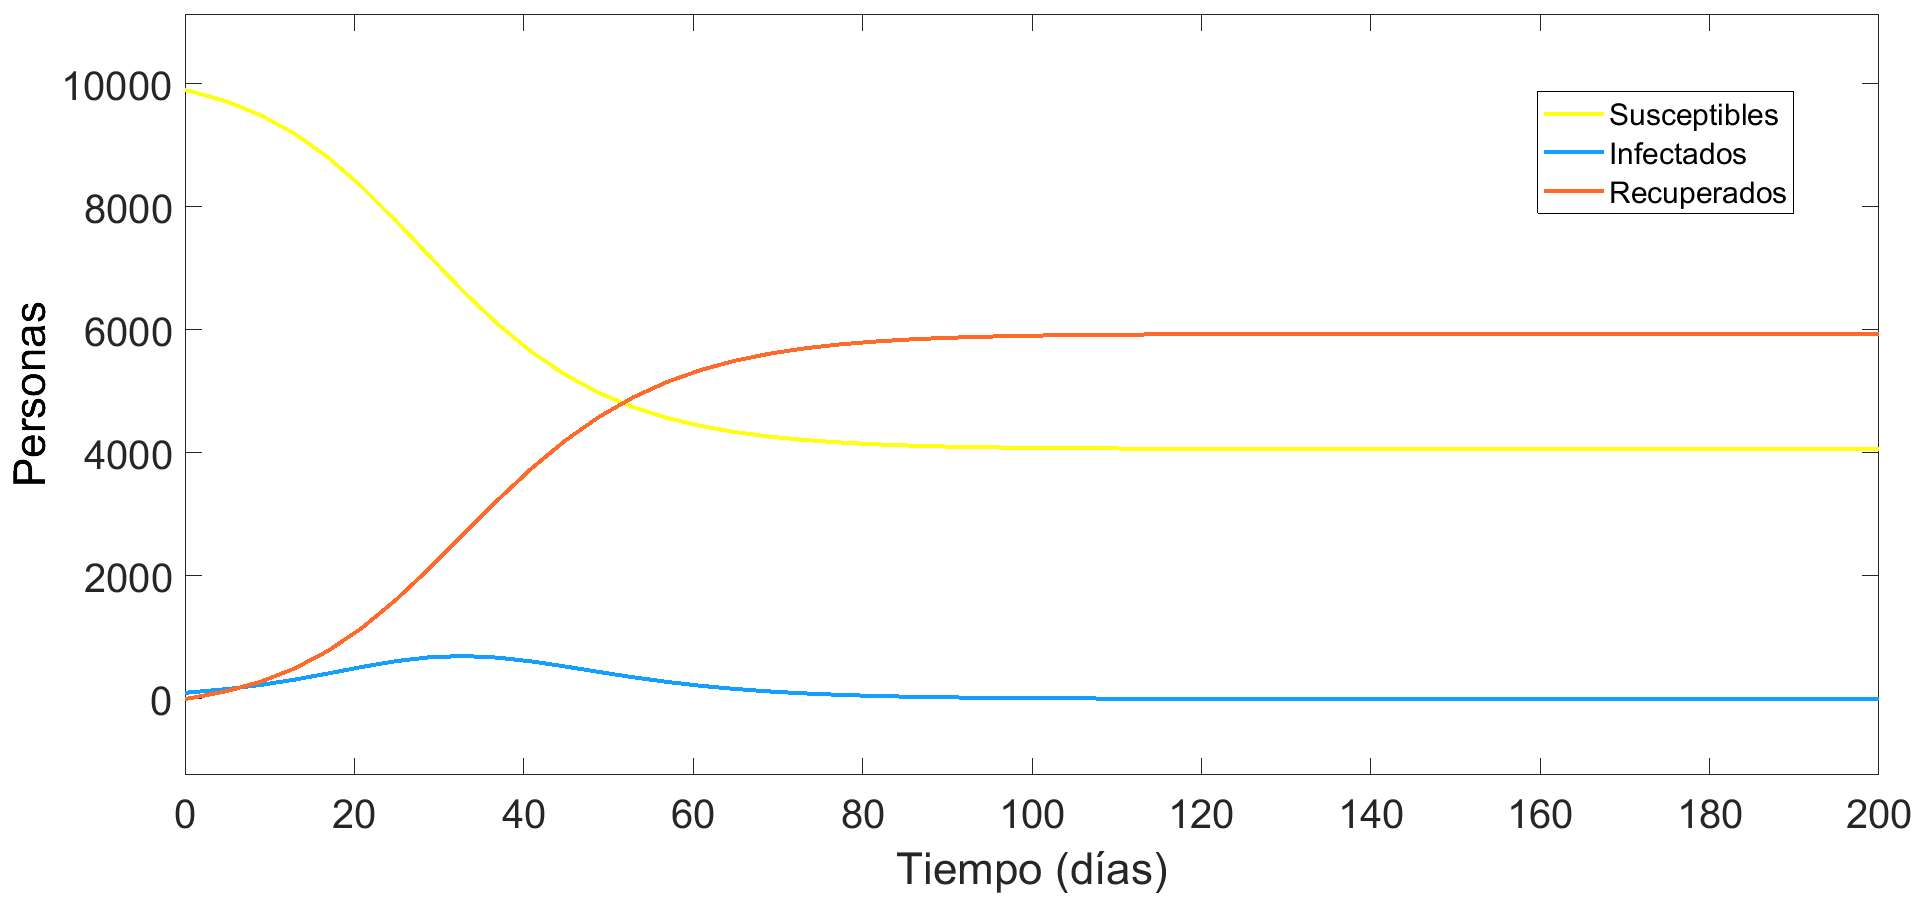
\includegraphics[width=0.7\textwidth]{img/modelo_SIR_32.png}
    \caption{Resultado modelo SIR con beta 0.0003 y gamma 0.2}
    \label{fig:Simulación 3 SIR}
    \vspace{0.5cm} % Ajusta el espacio vertical entre la imagen y el texto
\end{figure}

En la figura \ref{fig:Simulación 1 SIR}, la enfermedad se propaga lentamente pero de forma generalizada, todos los susceptibles acaban infectados y posteriormente recuperados. El pico de infecciones se da alrededor del día 100 con casi 6000 casos. El número básico de reproducción es 7, lo que explica la propagación total. Finalmente, la epidemia se extingue al no quedar susceptibles.
Para la figura \ref{fig:Simulación 3 SIR}, la enfermedad apenas se propaga, los infectados iniciales se recuperan rápidamente sin generar nuevos contagios significativos. La mayoría de la población permanece susceptible. El número básico de reproducción es 0,5, lo que indica que cada infectado contagia de media a menos de una persona. Esto provoca que el brote se extinga de forma rápida sin alcanzar una propagación masiva.
EN la última figura \ref{fig:Simulación 3 SIR} los susceptibles disminuyen lentamente y se estabilizan alrededor de 4000, lo que indica que una gran parte de la población no se infecta. El número de infectados crece levemente al inicio pero desciende rápidamente, y los recuperados aumentan hasta estabilizarse. La enfermedad se propaga de forma moderada, aunque el número básico de reproducción es 1,5, suficiente para permitir propagación, la epidemia no alcanza a toda la población y acaba desapareciendo con un brote limitado.

\subsection{Comportamiento modelo SIR con regulador PID}
Con el objetivo de mejorar el control sobre lo representado por el modelo SIR, se propone la implementación de un controlador PID. Este controlador permitirá ajustar dinámicamente una variable de control, la tasa de transmisión, en función del error entre el número actual de individuos infectados y un valor deseado (setpoint), que en este caso será de 1000 infectados. Para el diseño y ajuste del PID, se utilizarán los datos obtenidos previamente a partir de las simulaciones realizadas con el modelo SIR estándar, sin control. Estos datos permitirán identificar el comportamiento del sistema y evaluar la efectividad del controlador en mantener el número de infectados cercano al valor establecido.

En la figuras (\ref{fig:simu1pid})(\ref{fig:simu2pid})(\ref{fig:simu3pid}) se observan las simulaciones para el modelo SIR controlado con un regulador PID.

\begin{figure}[H]
    \centering
    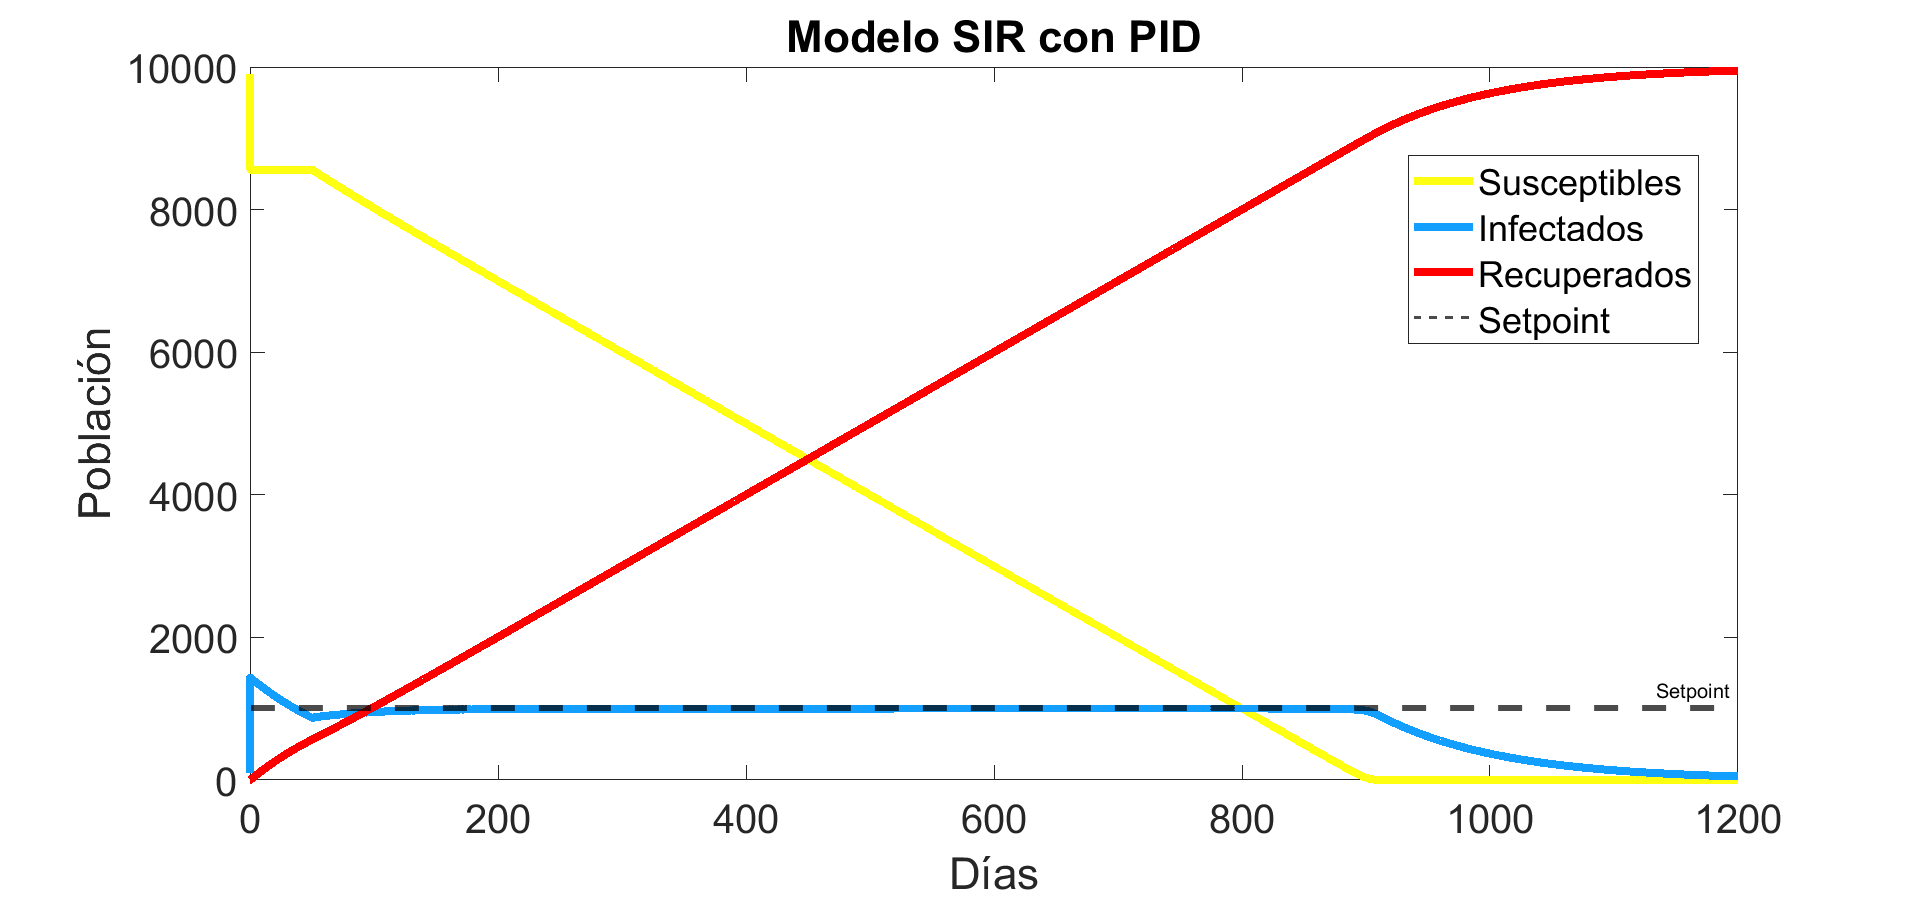
\includegraphics[width=0.7\textwidth]{img/modeloSIR_PID1.png}
    \caption{Simulación 1 para modelo SIR con PID, $\beta$ = 0.07 y $\gamma$ = 0.1}
    \label{fig:simu1pid}
    \vspace{0.5cm} % Ajusta el espacio vertical entre la imagen y el texto
\end{figure}

\begin{figure}[H]
    \centering
    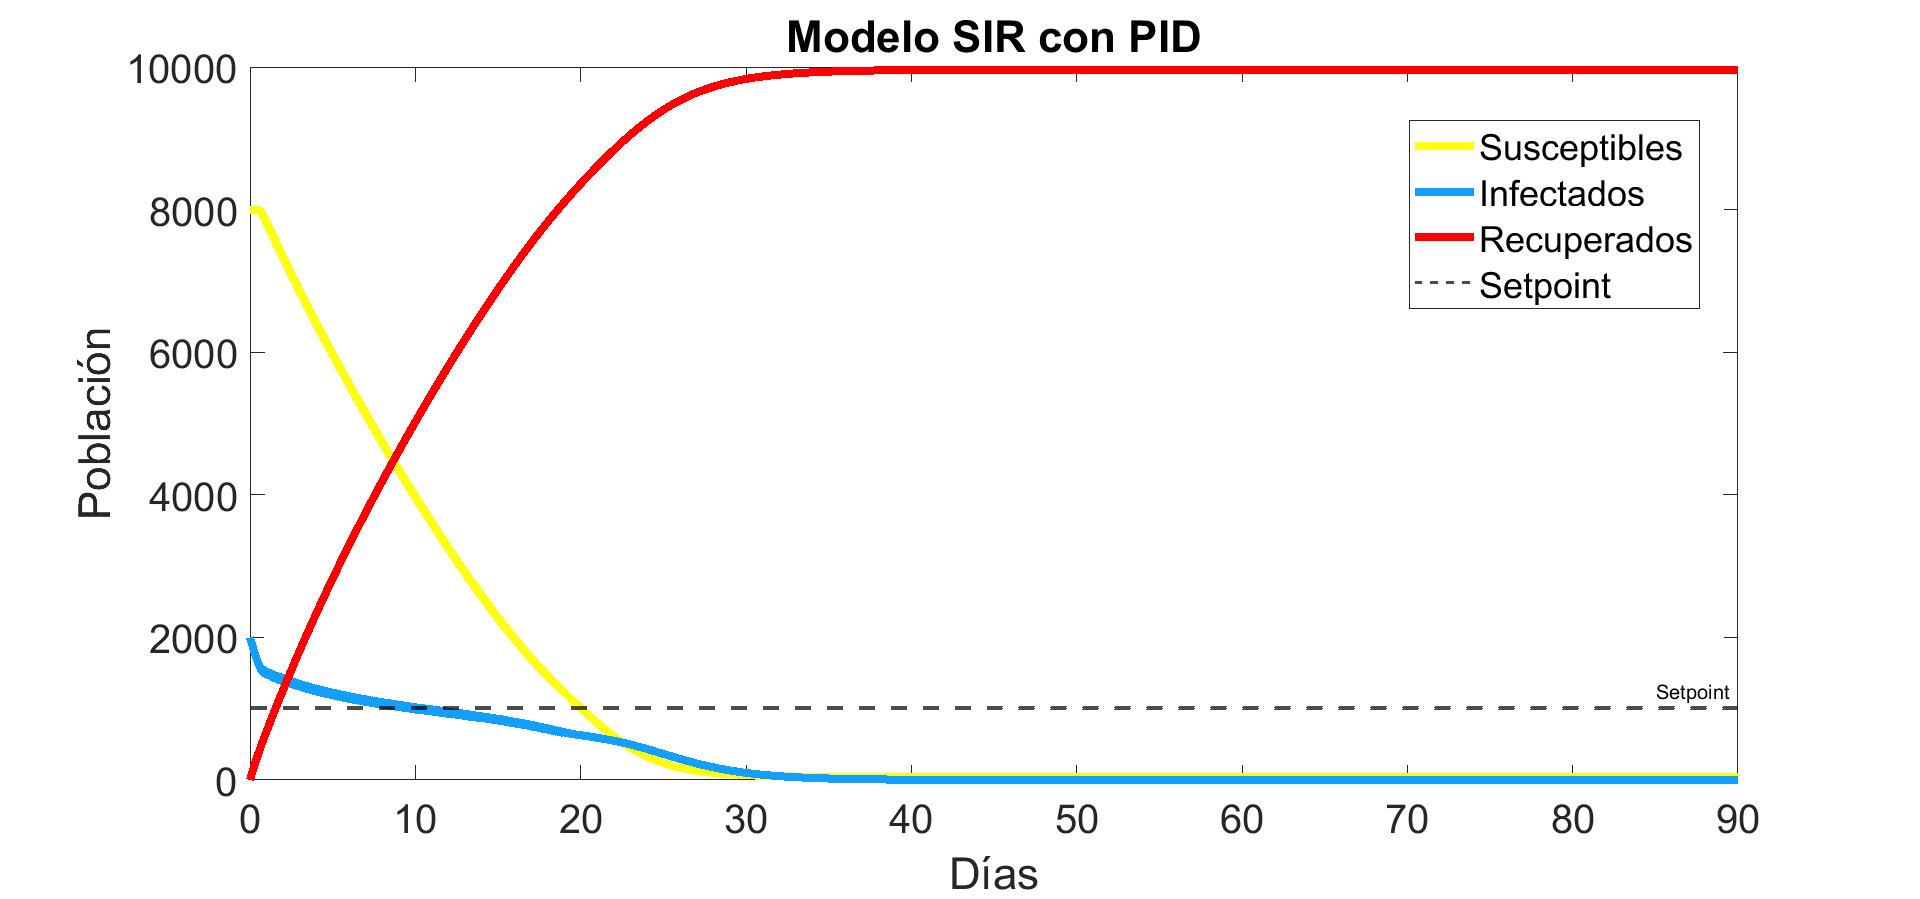
\includegraphics[width=0.7\textwidth]{img/modeloSIR_PID2.png}
    \caption{Simulación 1 para modelo SIR con PID, $\beta$ = 0.2 y $\gamma$ = 0.4}
    \label{fig:simu2pid}
    \vspace{0.5cm} % Ajusta el espacio vertical entre la imagen y el texto
\end{figure}

\begin{figure}[H]
    \centering
    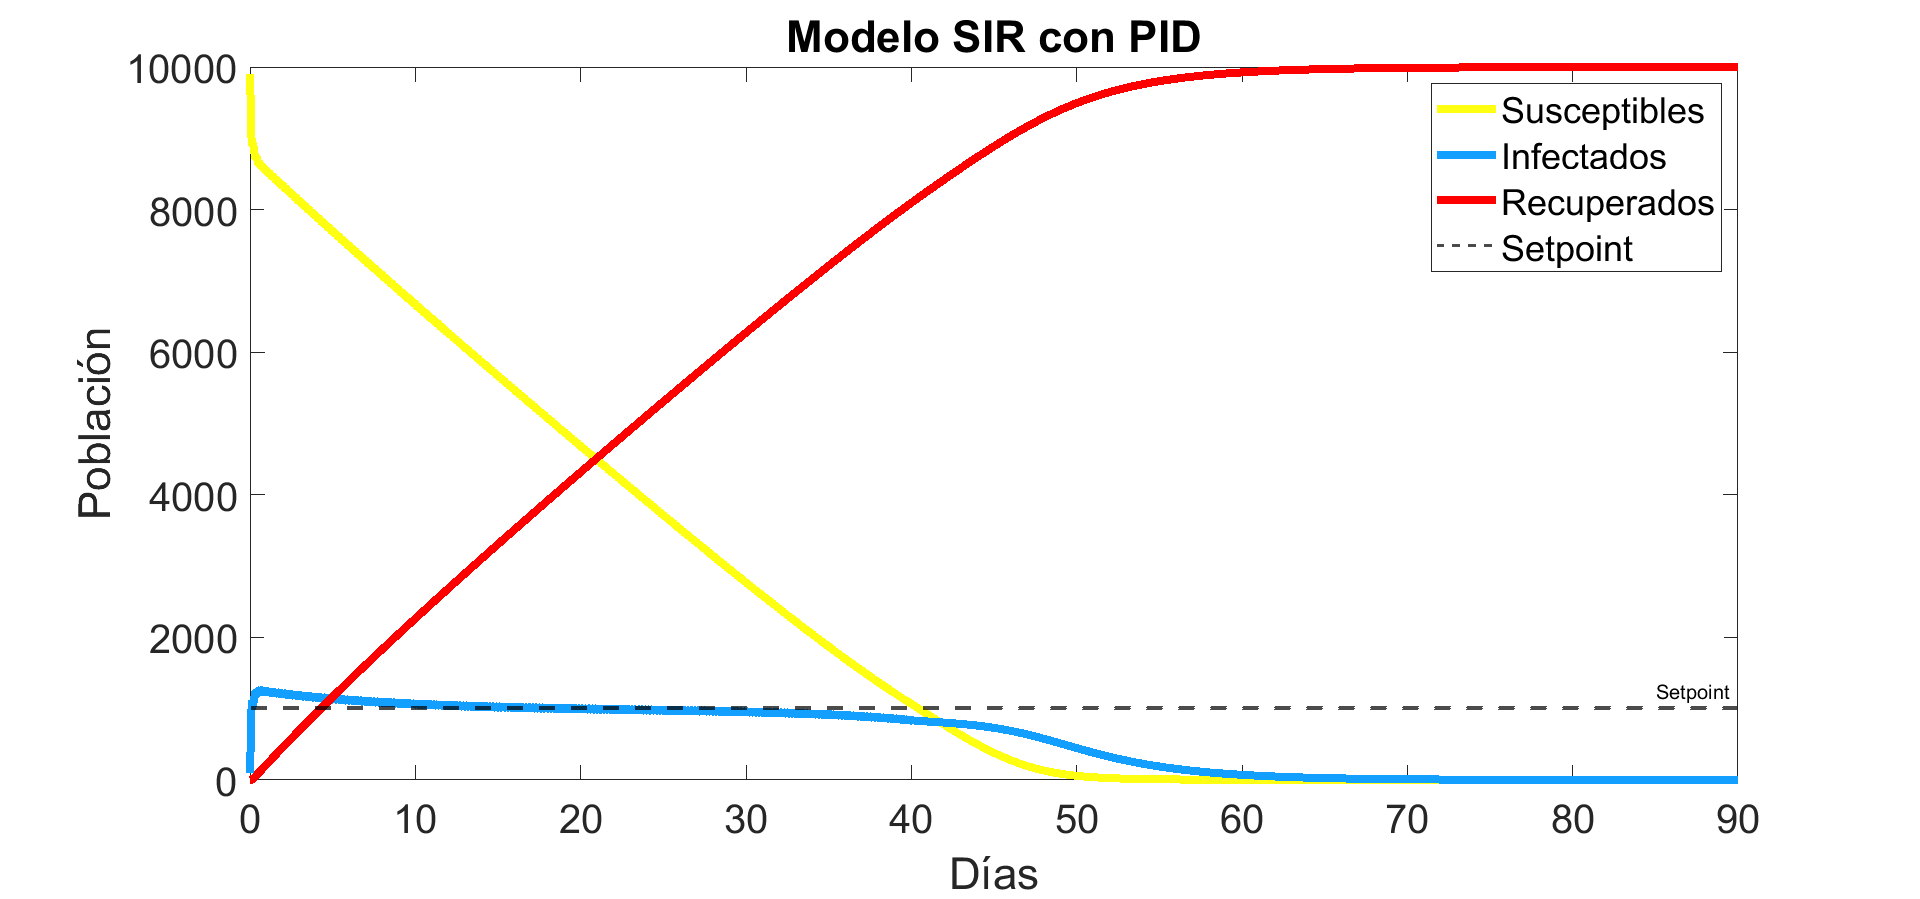
\includegraphics[width=0.7\textwidth]{img/modeloSIR_PID3.png}
    \caption{Simulación 1 para modelo SIR con PID, $\beta$ = 0.3 y $\gamma$ = 0.2}
    \label{fig:simu3pid}
    \vspace{0.5cm} % Ajusta el espacio vertical entre la imagen y el texto
\end{figure}

En la figura \ref{fig:simu1pid}, la enfermedad se propaga lentamente ya que el número de infectados crece de forma moderada y luego disminuye suavemente. En cuanto a los susceptibles bajan poco a poco, mientras que los recuperados aumentan gradualmente. El brote es controlado y no hay un pico muy alto. En la figura \ref{fig:simu2pid}, la infección se propaga más rápidamente, pero también hay una recuperación rápida. Se alcanza un pico alto de infectados en poco tiempo, luego desciende rápidamente.
Gran parte de la población termina recuperada en un tiempo corto. El proceso es más brusco, pero de corta duración. Y por últmo en cuanto a la figura\ref{fig:simu3pid}, se propaga muy rápido y con fuerza. El número de infectados crece rápidamente a un valor alto y tarda más en bajar, mientras que el número de susceptibles cae de manera abrupta. Se observa una epidemia fuerte y más prolongada.


\subsection{Comparación modelo SIR clásico y modelo SIR con regulador PID}
Para analizar el impacto del control sobre la evolución de una epidemia, se han comparado los resultados de simulaciones del modelo SIR con y sin la incorporación de un controlador PID. En ambos casos, se utilizaron los mismos valores para los parámetros $\beta$ y $\gamma$, permitiendo evaluar directamente el efecto del regulador sobre la dinámica del sistema.

Para la primera simulación con beta = 0.07 y gamma = 0.01, se observa que la propagación de la enfermedad es lenta debido a un valor muy bajo de $\beta$. En la figura \ref{fig:Simulación 1 SIR} sin PID, se observa que el número de infectados crece paulatinamente hasta alcanzar un pico considerable, y luego desciende lentamente a medida que más personas se recuperan. El sistema evoluciona de forma natural, sin intervención, y se aprecia un brote prolongado en el tiempo. En cambio, en la figura \ref{fig:simu1pid} con PID, el número de infectados se mantiene más contenido durante todo el proceso. El controlador actúa corrigiendo la tasa de contagio de forma dinámica, evitando que el pico de infectados sea muy alto. Además, la epidemia se resuelve en menos tiempo. Este caso demuestra que incluso en escenarios con transmisión lenta, el PID puede mejorar la respuesta del sistema al acelerar el descenso de los infectados y reducir la duración total del brote.

En cuanto a la segunda simulación con beta = 0.2 y gamma = 0.4, se plantea una tasa de recuperación elevada, lo que en teoría debería limitar la duración de la infección. En la simulación sin PID figura \ref{fig:Simulación 2 SIR}, el número de infectados aumenta inicialmente, pero se estabiliza en un valor constante. Este comportamiento sugiere que la enfermedad se vuelve endémica, manteniéndose presente en la población a lo largo del tiempo sin llegar a desaparecer del todo. Con el regulador PID activo figura \ref{fig:simu2pid}, el comportamiento cambia drásticamente. El número de infectados alcanza un valor cercano al setpoint y posteriormente disminuye hasta llegar prácticamente a cero. El controlador, al actuar sobre la tasa de contagio, permite reducir el número de infectados de manera más eficaz, eliminando la posibilidad de una infección sostenida en el tiempo. Esto pone en evidencia la capacidad del PID para forzar al sistema hacia un estado libre de infección, incluso cuando la dinámica natural tiende al equilibrio.

\subsection{Comportamiento epidemia sarampión}
Se simula el comportamiento de la enfermedad del sarampión, utilizando los datos definidos anteriormente en el apartado de descripción de los datos. La figura \ref{fig:simusara} muestra la evolución del sarampión.

\begin{figure}[H]
    \centering
    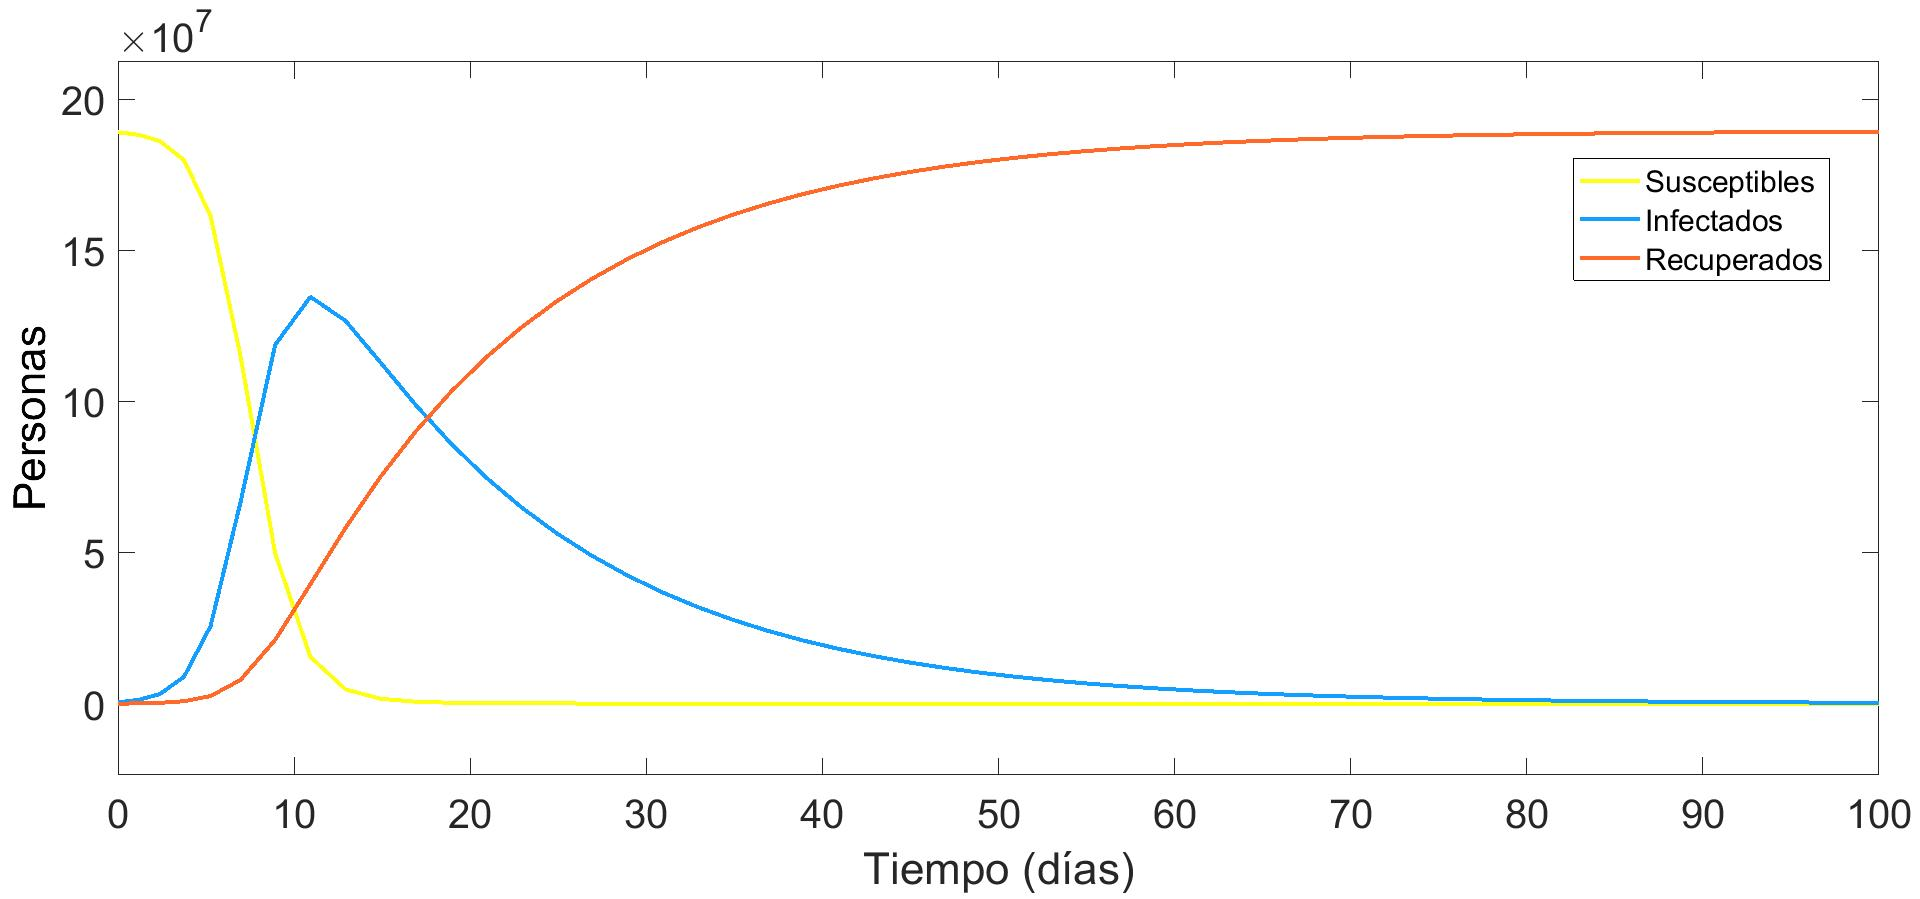
\includegraphics[width=0.7\textwidth]{img/modelo_SIR.jpg}
    \caption{Resultado modelo SIR con datos reales para el sarampión}
    \label{fig:simusara}
    \vspace{0.5cm} % Ajusta el espacio vertical entre la imagen y el texto
\end{figure}

En la gráfica (\ref{fig:simusara}) obtenida se refleja claramente el comportamiento típico de una enfermedad infecciosa altamente contagiosa, y más si no hay medidas de control como la vacuna.
Al principio, la mayor parte de la población se encuentra en el grupo de susceptibles. Sin embargo, debido al gran valor de $R_0$, la enfermedad se propaga con rapidez. Como consecuencia los susceptibles descienden bruscamente en los primero días, un gran número de personas contrae la enfermedad en un corto periodo de tiempo. Posteriormente, la curva llega a cero, que refleja que toda la población se ha infectado.
En cuanto a los infectados, la curva presenta un crecimiento rápido al principio de la epidemia, alcanzando un pico endémico sobre el día 12. En este punto se registra el número máximo de personas infectadas de forma simultánea. Tras este pico, los infectados empiezan a disminuir progresivamente. Esto es debido a que las personas se recuperan y pasan al compartimento de los recuperados, y además quedan muy pocos susceptibles, por lo que la transmisión se ralentiza hasta que se detiene.
Por otro lado, los recuperados van creciendo sostenidamente en el tiempo, empezando en cero y creciendo de forma acelerada en un principio. A medida que los infectados se recuperan, la curva sube hasta que toda la población ha superado la enfermedad y ha adquirido inmunidad permanente. Cuando la curva de los recuperados se estabiliza indica que la epidemia ha llegado a su fin, porque no quedan personas susceptibles que puedan volver a infectarse.

\subsection{Comportamiento del sarampión tras la vacunación}
Para este modelo, los datos también se han explicado en el apartado de descripción de los datos. Son los mismos que para sin vacunación, lo que pasa que se añade la tasa de vacunación ahora. La figura \ref{fig:simu saramp vacuna} muestra la evolución del sarampión pero contando que ahora se ha introducido como medida de control la vacunación.

\begin{figure}[H]
    \centering
    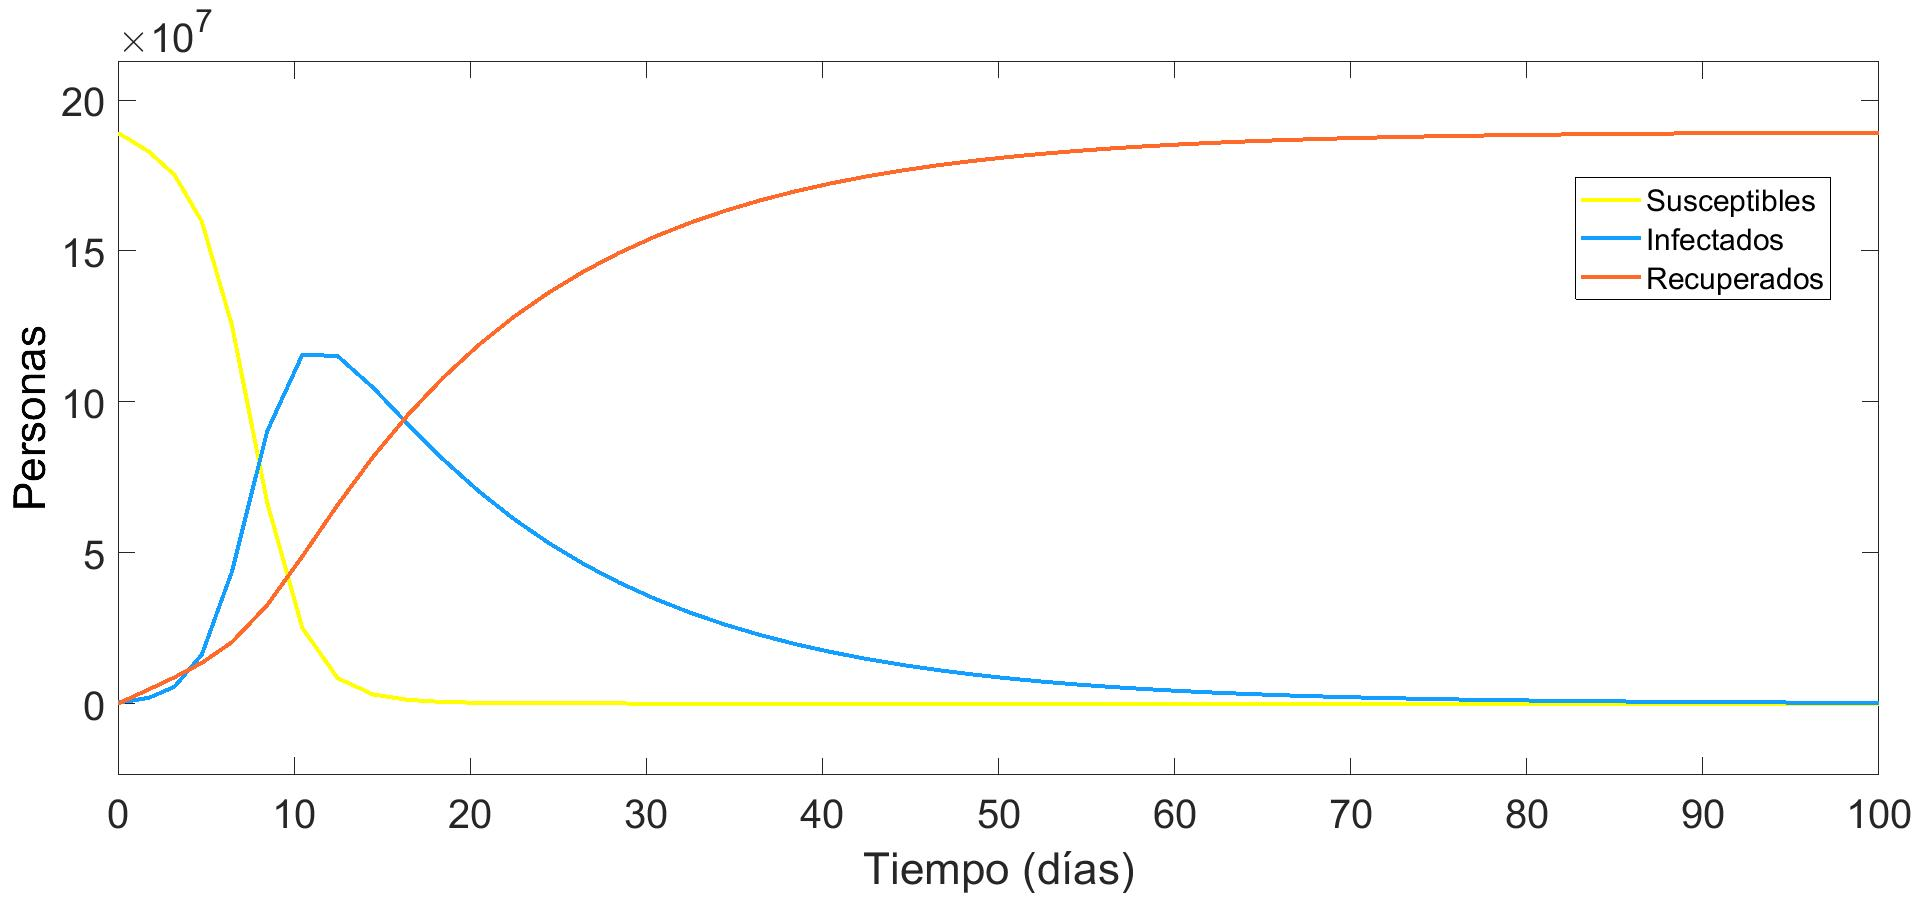
\includegraphics[width=0.7\textwidth]{img/modelo_SIRV_inicio.jpg}
    \caption{Resultado modelo SIRV con datos reales para el sarampión, con medida de control de vacunación}
    \label{fig:simu saramp vacuna}
    \vspace{0.5cm} % Ajusta el espacio vertical entre la imagen y el texto
\end{figure}

En la gráfica \ref{fig:simu saramp vacuna} las personas susceptibles descienden muy rápido en los primero días, más pronunciado que la simulación sin vacunación. Se debe a que gran parte de los susceptibles son vacunados directamente, lo que reduce la cantidad de personas expuestas al contagio. Prácticamente en los primeros días desaparece el grupo de susceptibles, lo que limita la propagación del virus.
En cuanto a los infectados, aunque se alcanza un pico de infecciones, es más bajo que en la simulación sin vacunación. Se sitúa en torno a 11 millones de infectados, además se produce más temprano, que indica que el brote es más contenido y se disipa más rápido por la inmunidad inducida por la vacunación.
Mientras que el número de recuperados crece rápidamente desde los primeros días. A diferencia del modelo sin vacunación, donde el crecimiento del grupo recuperado dependía únicamente de las personas que superaban la enfermedad, en esta simulación también se incluyen los vacunados, que pasan directamente a este compartimento. Por ello, la curva de recuperados comienza a crecer antes y con mayor pendiente, alcanzando valores más altos en menos tiempo y reflejando una inmunidad colectiva mucho más rápida.

La comparación entre ambas simulaciones muestra claramente que la introducción de la vacunación masiva es altamente efectiva para contener la propagación del sarampión. Reduce significativamente el número de casos, la duración del brote y la exposición de la población susceptible. Esto evidencia la importancia de las campañas de vacunación como herramienta clave de salud pública, especialmente frente a enfermedades con un número básico de reproducción elevado como el sarampión.




\section{Comportamiento modelo SEIR}
Para el modelo SEIR se han realizado varias simulaciones con valores distintos. Los datos que se utilizan se encuentran en la tabla \ref{tab:datos para modelo SEIR}.

\begin{table}[H]
\centering
\begin{tabular}{|c|c|c|c|}
\hline
\textbf{Parámetro} & \textbf{Simulación 1} & \textbf{Simulación 2}  & \textbf{Simulación 3}\\
\hline
Susceptibles (S) & 9900 & 8000 & 9900\\
\hline
Expuestos (R)   &  0   & 0 & 0  \\
\hline
Infectados (I)   & 100   & 2000 & 100  \\
\hline
Recuperados (R)   &  0   & 0 & 0  \\
\hline
\(\beta\)        & 0.0001 & 0.0001  & 0.0006\\
\hline
\(\sigma\)        & 0.1 & 0.2  & 0.3\\
\hline
\(\gamma\)        & 0.05 & 0.1 & 0.1\\
\hline
\end{tabular}
\caption{Datos usados para ver el comportamiento del modelo SEIR}
\label{tab:datos para modelo SEIR}
\end{table}

Se observan los resultados para cada simulaación en las figuras siguientes (\ref{fig:Simulación 1 SEIR})(\ref{fig:Simulación 2 SEIR})(\ref{fig:Simulación 3 SEIR}).

\begin{figure}[H]
    \centering
    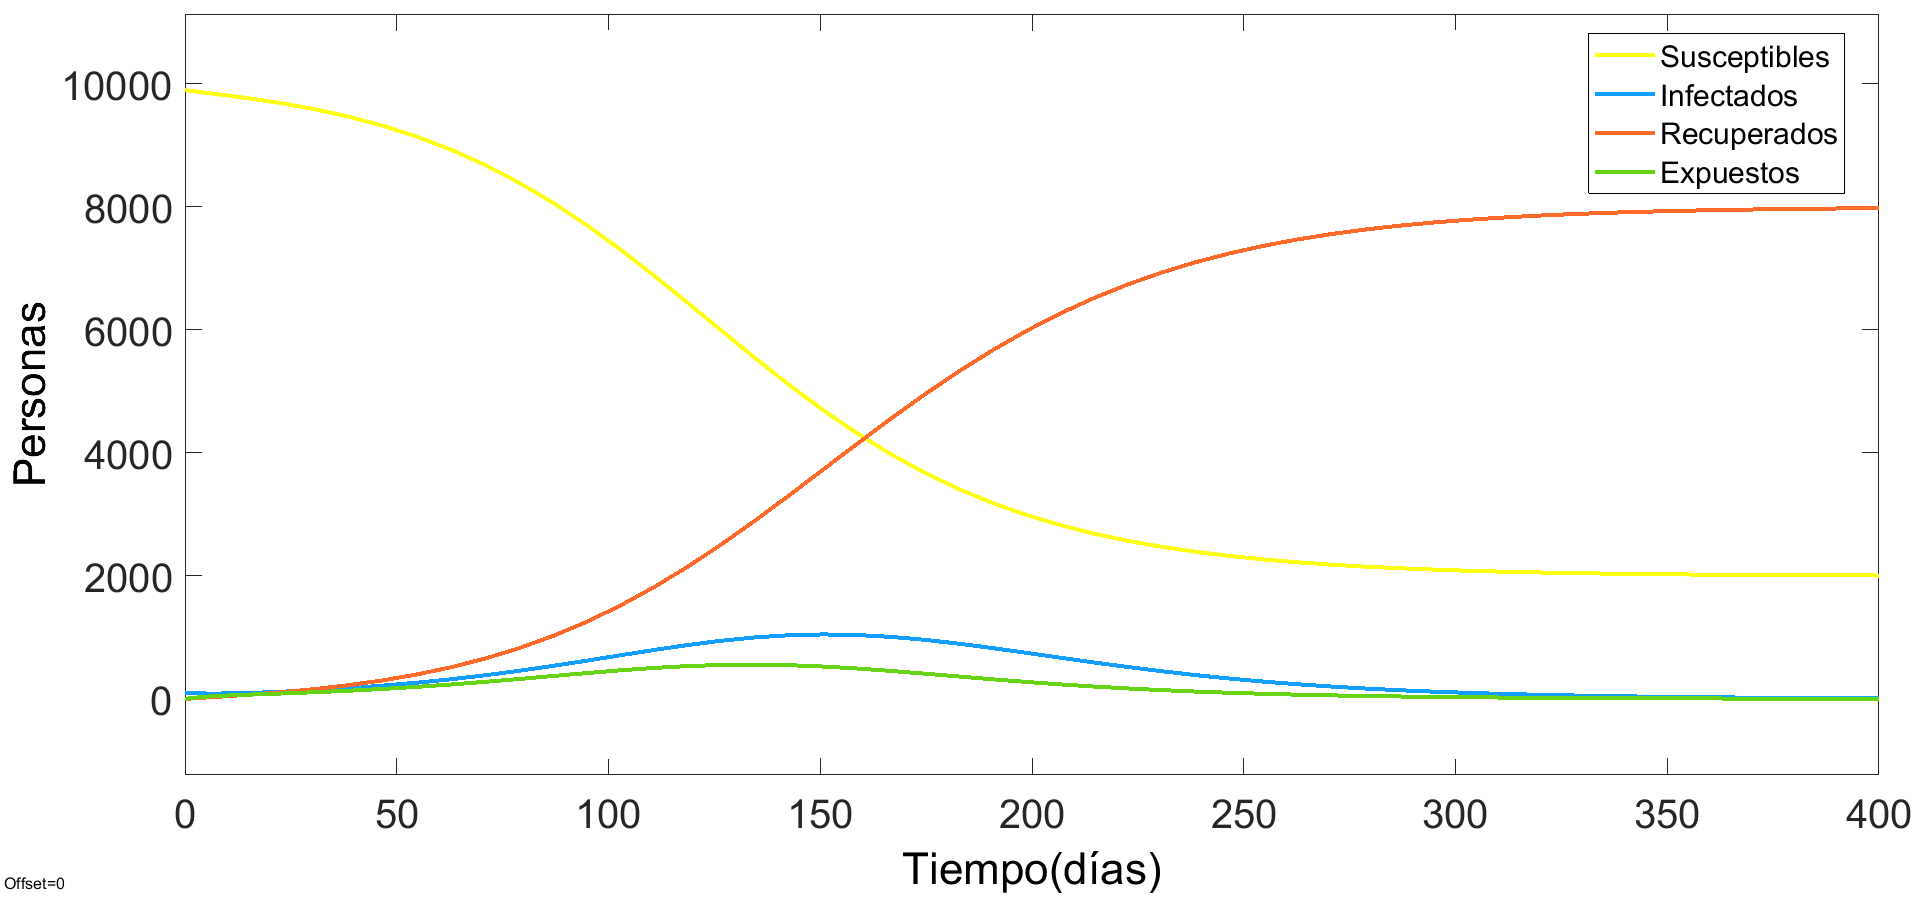
\includegraphics[width=0.7\textwidth]{img/modelo_SEIR_1105.png}
    \caption{Resultado modelo SEIR con beta 0.0001, sigma 0.1 y gamma 0.05}
    \label{fig:Simulación 1 SEIR}
    \vspace{0.5cm} % Ajusta el espacio vertical entre la imagen y el texto
\end{figure}

\begin{figure}[H]
    \centering
    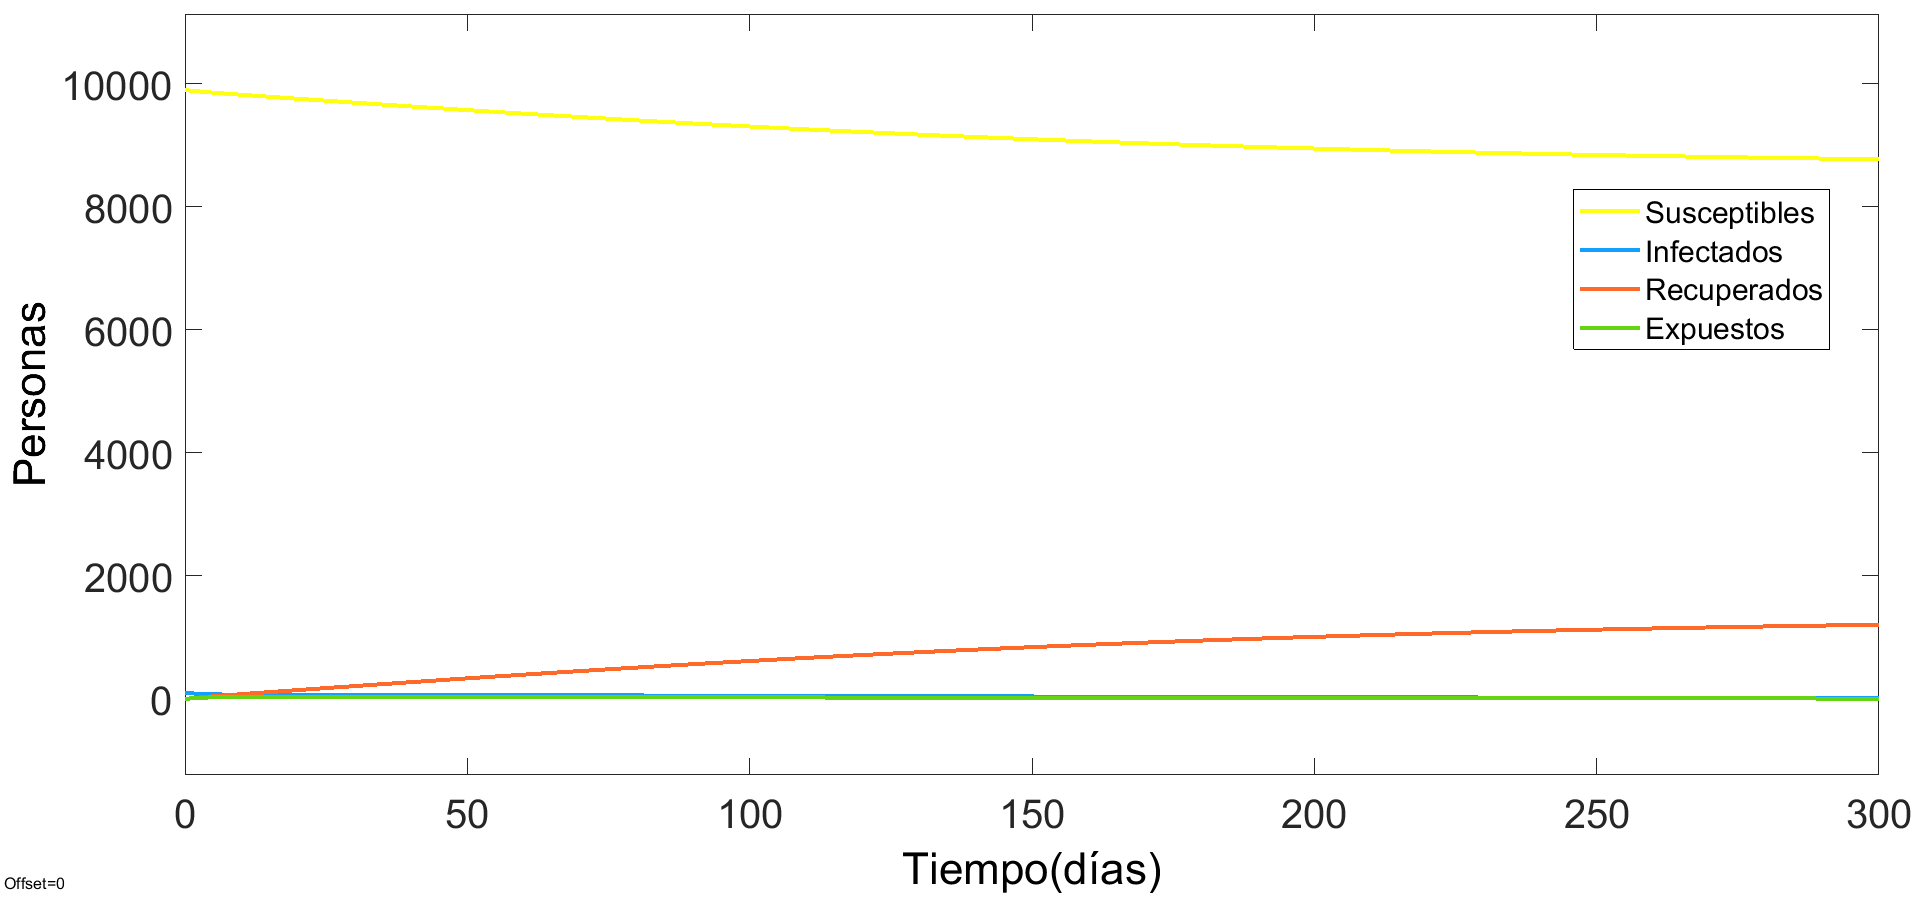
\includegraphics[width=0.7\textwidth]{img/modelo_SEIR_121.png}
    \caption{Resultado modelo SEIR con beta 0.0001, sigma 0,2 y gamma 0.1}
    \label{fig:Simulación 2 SEIR}
    \vspace{0.5cm} % Ajusta el espacio vertical entre la imagen y el texto
\end{figure}

\begin{figure}[H]
    \centering
    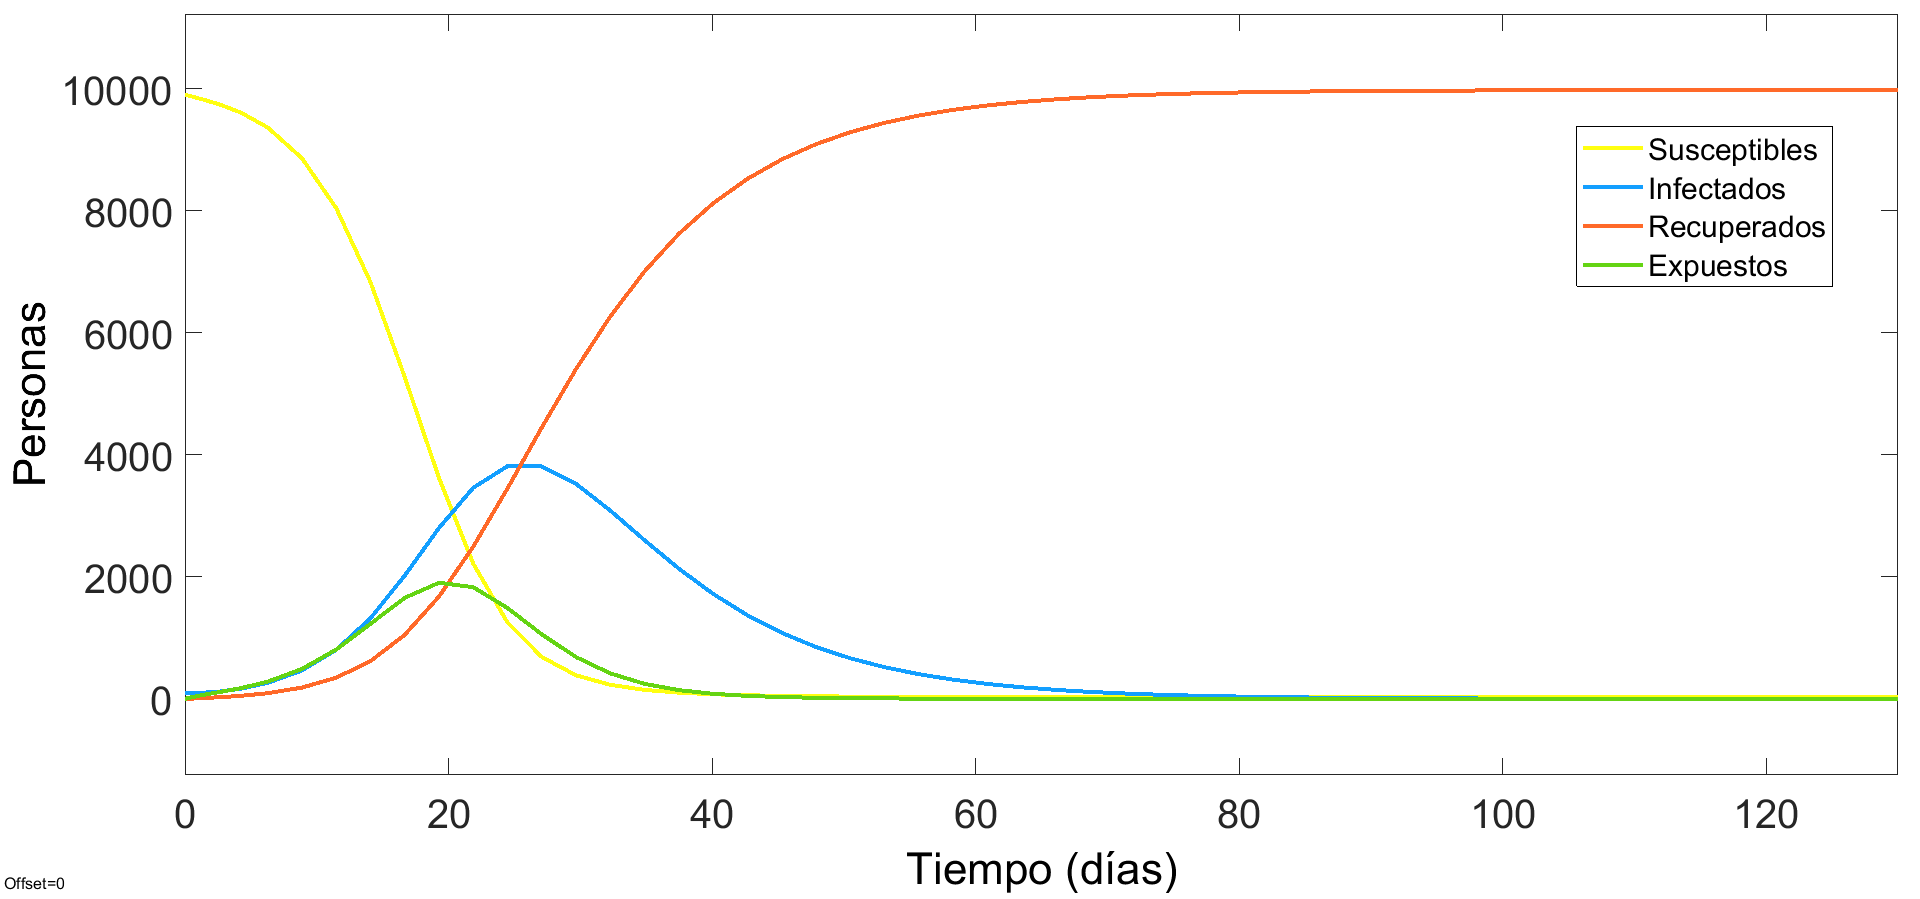
\includegraphics[width=0.7\textwidth]{img/modelo_SEIR_631.png}
    \caption{Resultado modelo SEIR con beta 0.0006, sigma 0,3 y gamma 0.01}
    \label{fig:Simulación 3 SEIR}
    \vspace{0.5cm} % Ajusta el espacio vertical entre la imagen y el texto
\end{figure}

En la primera gráfica \ref{fig:Simulación 1 SEIR} el número de personas expuestas crece inicialmente y luego decrece. Los infectados presentan un pico, moderado, debido a la baja tasa de transmisión y la recpueración lenta. Los recuperados aumentan progresivamente. Los susceptibles descienden de manera paulatina. En cuanto a la gráfica \ref{fig:Simulación 2 SEIR}, a pesar de que el paso es más rápido de expuestos a infectados y hay mayor tasa de recuperación, el número de infectados se mantiene muy bajo. El brote está contenido, sin un pico relevante. Gran parte de la población sigue siendo susceptible, con pocos recuperados. El sistema se mantiene estable, no hay propagación significativa. Por último la figura \ref{fig:Simulación 3 SEIR}. El sistema reacciona con una rápida propagación, habiendo un pico marcado de infectados.
La mayoría de la población pasa a la categoría de recuperados.
Los susceptibles caen bruscamente, mostrando que la infección se ha propagado de forma extensa.





\subsection{Comportamiento pandemia COVID-19}
Se simula el comportamiento de la enfermedad del sarampión, utilizando los datos definidos anteriormente en el apartado de descripción de los datos. La figura \ref{fig:Simucov} muestra la evolución del COVID-19 en España desde su inicio.

\begin{figure}[H]
    \centering
    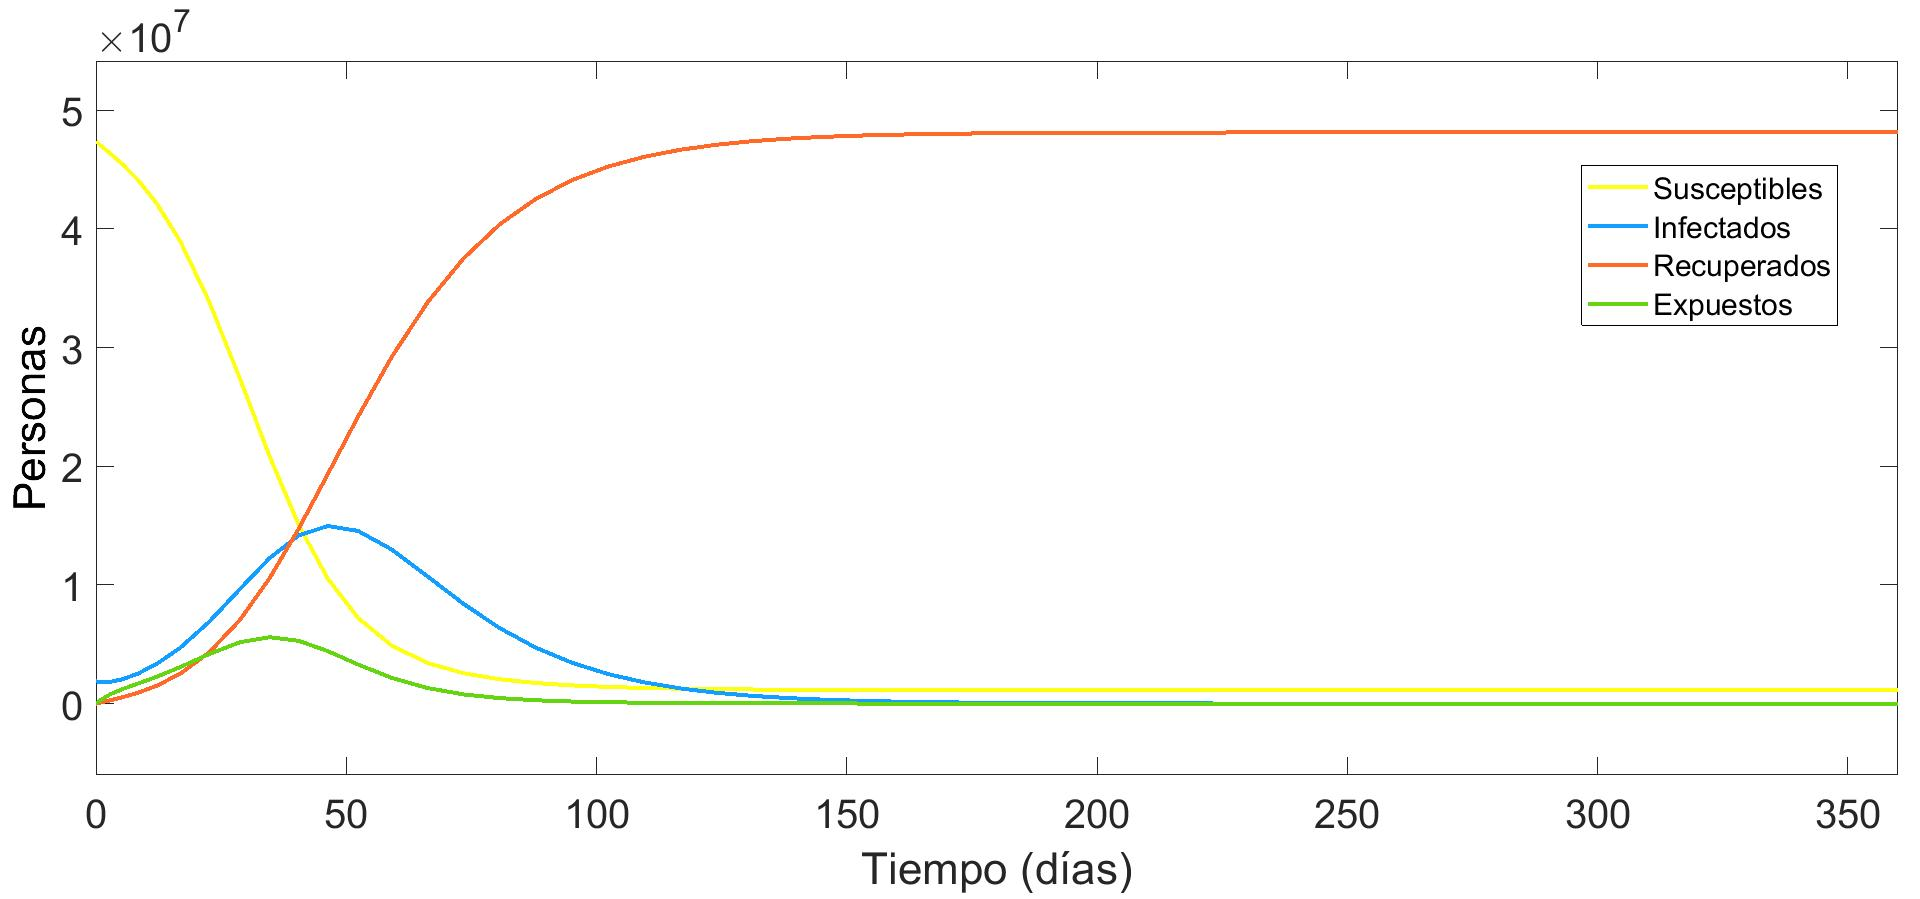
\includegraphics[width=0.7\textwidth]{img/modelo_SEIR.jpg}
    \caption{Resultado modelo SEIR con datos reales para el COVID-19}
    \label{fig:Simucov}
    \vspace{0.5cm} % Ajusta el espacio vertical entre la imagen y el texto
\end{figure}

En la simulación \ref{fig:Simucov} se pueden obtener las siguientes observaciones. La población susceptible disminuye rápidamente, al inicio prácticamente la mayoría de la población era susceptible. mientras avanza el tiempo, disminuyen de manera pronunciada, debido al contacto entre las personas debido al contacto entre personas infectadas. La curva se estabiliza, gran parte de la población se ha contagiado, pero siguen quedando personas susceptibles.
La curva de los expuestos presenta un crecimiento inicial que se adelanta a la curva de los infectados, lo cual es coherente con este modelo, ya que las personas primero pasan por el periodo de incubación antes de convertirse en transmisores activos. El pico de personas infectadas se alcanza alrededor del día 50 aproximadamente, en este momento se observa mayor número de casos activos simultáneos. La curva desciende ya que los infectados se recuperan y los susceptibles disminuyen.
La curva de los recuperados mantiene un crecimiento constante, que se acelera con el pico de infecciones. Hacia el final de la simulación, la mayoría de la población se encuentra en el compartimento de recuperados, indica que la enfermedad ha dejado de propagarse de forma activa por falta de individuos susceptibles.
Aproximadamente a partir del día 150, el sistema entra en una fase de estabilidad. Los valores de todos los compartimentos se estabilizan, y prácticamente no hay nuevos contagios.  La enfermedad ha agotado su capacidad de transmisión debido a que casi toda la población ha adquirido inmunidad.
El retraso entre las curvas de expuestos e infectados muestra claramente el efecto del periodo de latencia. Este desfase temporal tiene consecuencias importantes desde el punto de vista epidemiológico, ya que dificulta la detección temprana de brotes y puede permitir la transmisión antes de que se manifiesten los síntomas.

\subsection{Comportamiento COVID-19 con vacunación}
Para este modelo, los datos también se han explicado en el apartado de descripción de los datos. Son los mismos que para sin vacunación, lo que pasa que se añade la tasa de vacunación. La figura \ref{fig:Simucov vacunacion} muestra la evolución del sarampión

\begin{figure}[H]
    \centering
    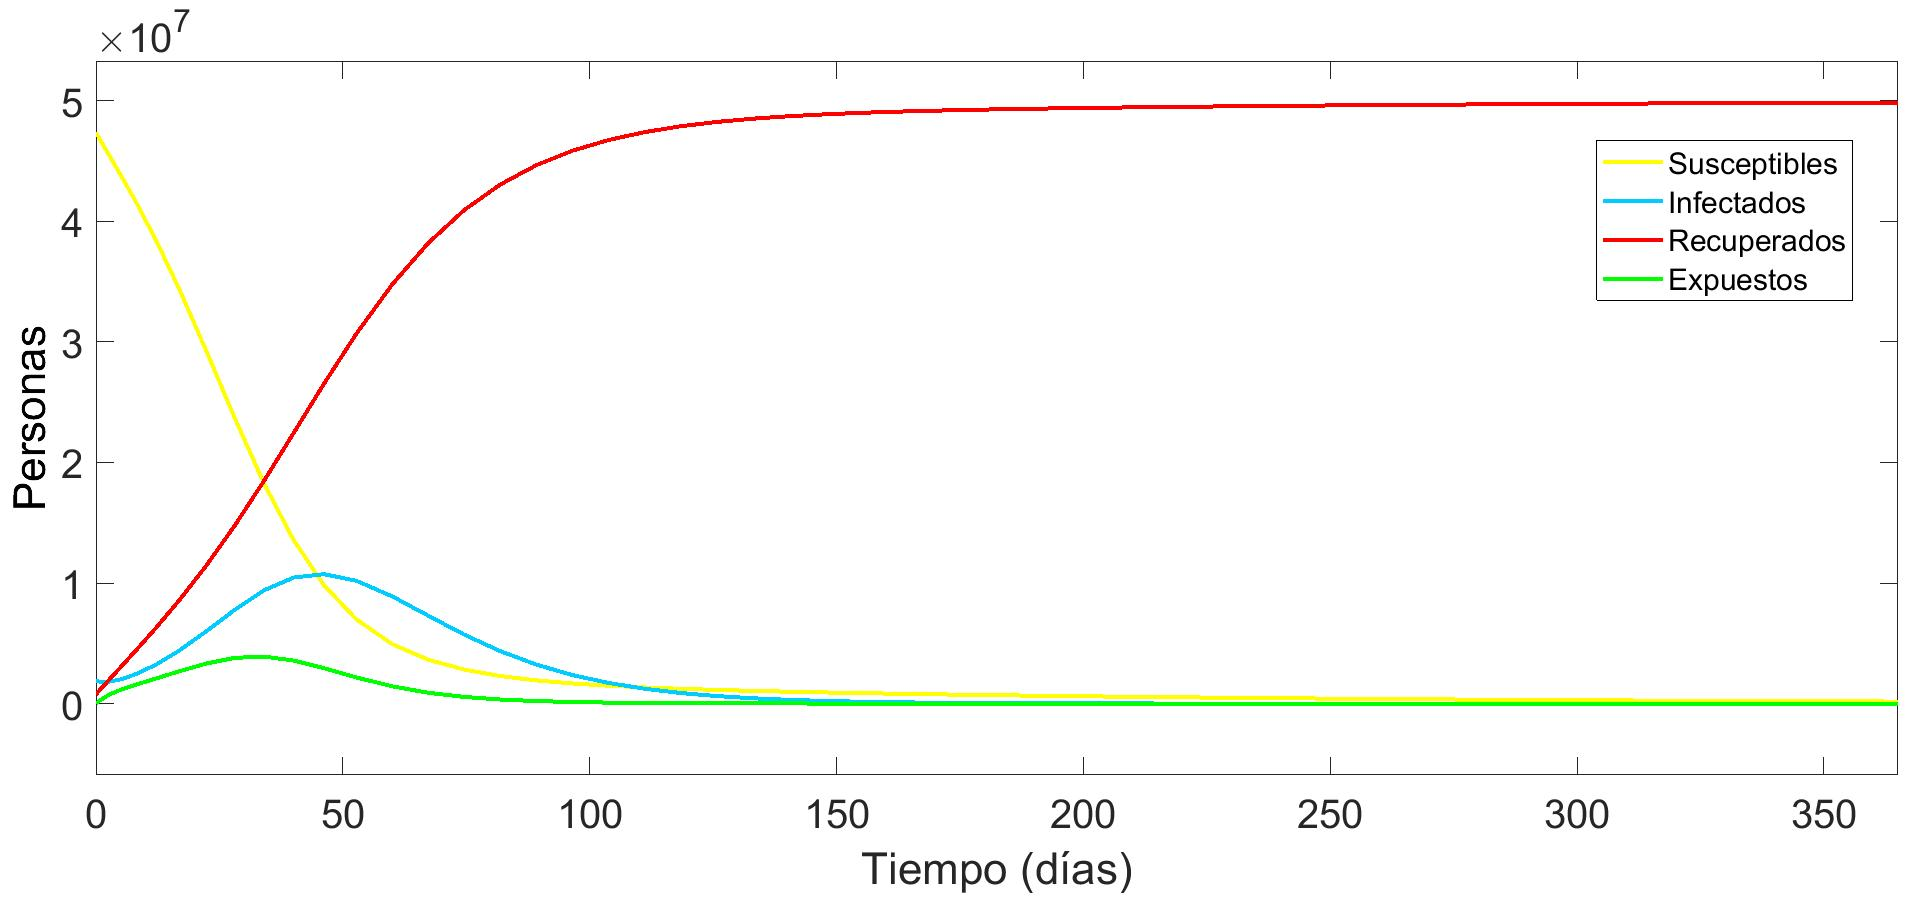
\includegraphics[width=0.7\textwidth]{img/modelo_SEIRV.jpg}
    \caption{Resultado modelo SEIRV con datos reales para el COVID-19, con medida de control de vacunación}
    \label{fig:Simucov vacunacion}
    \vspace{0.5cm} % Ajusta el espacio vertical entre la imagen y el texto
\end{figure}

Tras implementar el modelo SEIRV con la incorporación de la vacunación masiva en la población, se puede observar un cambio sustancial en la evolución de la epidemia de COVID-19 respecto al modelo SEIR sin vacunación \ref{fig:Simucov vacunacion}.
En la gráfica obtenida con el modelo SEIRV, se aprecia cómo el número de infectados alcanza un pico considerablemente menor y de menos duración en comparación con la simulación sin vacunación. Este resultado evidencia que la campaña de vacunación contribuye significativamente a reducir la carga máxima del sistema sanitario, evitando un colapso en momentos críticos.
El número de susceptibles disminuye rápidamente debido a dos factores: el contagio y la vacunación. A diferencia del modelo sin vacunación, donde la disminución se debía únicamente a la transmisión del virus, en este caso parte de la población abandona el estado de susceptible al recibir la vacuna y se incorpora directamente al compartimento de recuperados, sin haber pasado por la enfermedad, pero con la misma inmunidad que las personas que han pasado la enfermedad.
La curva de recuperados muestra un crecimiento más rápido y sostenido gracias al efecto de la vacunación, alcanzando antes un número elevado de personas inmunes. Esto acelera la inmunidad colectiva, lo que a su vez disminuye la probabilidad de nuevos contagios en fases posteriores.
Asimismo, la curva de expuestos, representa a aquellos que han estado en contacto con el virus pero aún no son contagiosos, muestra un comportamiento más controlado, evitando una acumulación excesiva de casos latentes como ocurría en la simulación sin vacunación.
Comparando ambos modelos, se concluye que la vacunación tiene un impacto clave en:
\begin{itemize}
    \item Disminuir el número total de personas infectadas.
    \item Reducir la velocidad de propagación.
    \item Limitar el número de personas susceptibles en el tiempo.
    \item Acelerar el final de la epidemia al aumentar rápidamente el número de recuperados.
\end{itemize}	
Estos resultados reflejan de forma cuantitativa cómo una campaña de vacunación masiva, como la que se implementó en España a partir de diciembre de 2020, puede modificar de manera muy significativa la evolución de una pandemia, confirmando la eficacia de esta estrategia como medida de control sanitario.



\section{Discusión}
\textbf{Modelo SI}. Los resultados muestran que cuando el valor de $\beta$ es elevado, el número de contagios crece rápidamente. Esto se debe a que cada encuentro entre una persona infectada y una susceptible tiene una alta probabilidad de resultar en un nuevo caso. Como consecuencia, la epidemia se desarrolla en un corto periodo de tiempo y afecta a un gran número de personas en fases tempranas del brote. En estos casos, la enfermedad puede propagarse de forma explosiva, reduciendo drásticamente el margen de actuación para implementar medidas de contención.
Por el contrario, cuando $\beta$ es bajo, la probabilidad de que un contacto provoque un contagio disminuye. Esto reduce la expansión del brote, permitiendo que el número de infectados crezca de forma más gradual. En este escenario, aunque la enfermedad puede seguir extendiéndose, lo hace a un ritmo más lento, lo que facilita la intervención temprana y el control del brote.
Estimar con precisión el valor de $\beta$ es fundamental para diseñar medidas de control adecuadas desde el inicio del brote.
Se puede concluir:
\begin{itemize}
    \item A mayor valor de $\beta$, mayor será la velocidad de propagación de la enfermedad.
    \item Una $\beta$ baja ralentiza el brote, permitiendo una intervención más efectiva.
\end{itemize}

\vspace{2em} 

\textbf{Modelo SI, SIDA/VIH}. Cabe destacar que el modelo SI utilizado en esta simulación representa una idealización de la dinámica de transmisión del VIH, y aunque resulta útil para comprender el comportamiento general de la enfermedad, no refleja con total precisión la complejidad de su propagación en la realidad.
El VIH es una enfermedad de transmisión sexual, lo que implica que no toda la población tiene el mismo nivel de riesgo de contagio. En la práctica, la probabilidad de transmisión varía considerablemente en función de factores como el comportamiento sexual, el acceso a educación sexual, el uso de métodos de protección (como preservativos), el número de parejas sexuales, el nivel de conciencia pública sobre la enfermedad y el acceso a servicios sanitarios.
Además, a diferencia del modelo SI que asume una transmisión homogénea en toda la población, en la vida real existen grupos poblacionales con mayor o menor exposición al virus, como pueden ser los trabajadores sexuales, personas que consumen drogas inyectables, o quienes tienen relaciones sexuales sin protección. Esto genera una heterogeneidad en la dinámica del contagio que no está reflejada en un modelo tan simplificado.

Por otro lado, la implementación de medidas de control y prevención (como campañas de concienciación, distribución de preservativos, pruebas de diagnóstico y tratamientos antirretrovirales) puede alterar significativamente la evolución del brote. Si bien el modelo SI predice una propagación continua e irreversible, en contextos reales estas medidas pueden frenar e incluso estabilizar el número de casos, impidiendo que toda la población se infecte.
Por tanto, aunque el modelo SI ofrece una buena aproximación teórica para enfermedades crónicas como el VIH, es fundamental interpretar los resultados con cautela y considerar las particularidades sociales, biológicas y conductuales que influyen en la propagación del virus en la vida real.
\vspace{2em}

\textbf{Modelo SIS}.
Las simulaciones han permitido observar cómo la evolución de la enfermedad está determinada principalmente por dos parámetros fundamentales:
\begin{itemize}
    \item Tasa de transmisión ($\beta$): representa la facilidad con la que se transmite la enfermedad. Un valor elevado implica una rápida propagación, especialmente en las fases iniciales del brote, cuando la mayoría de la población es susceptible. A medida que el número de infectados aumenta, los contagios se aceleran significativamente.
    \item Tasa de recuperación ($\gamma$): indica la velocidad con la que los individuos infectados se recuperan y vuelven a ser susceptibles. Cuanto mayor es, menor es el tiempo durante el cual una persona puede contagiar, lo que contribuye a frenar la propagación de la enfermedad.
\end{itemize}
La interacción entre estos dos parámetros se resume en el número básico de reproducción, $R_0$, que es clave para predecir el comportamiento del brote:
\begin{itemize}
    \item Si $R_0$ < 1, la enfermedad no logra propagarse de manera efectiva. Cada infectado contagia, de media, a menos de una persona, por lo que el número de infectados disminuye con el tiempo y la enfermedad desaparece.
    \item Si $R_0$ > 1, se produce un brote epidémico. La enfermedad persiste en el tiempo y se alcanza un equilibrio endémico, en el que las infecciones se compensan con las recuperaciones. La población mantiene de forma constante una proporción de individuos infectados y susceptibles.
\end{itemize}
Una de las observaciones más relevantes de las simulaciones es que la enfermedad no afecta a toda la población simultáneamente. Debido a la naturaleza del modelo, los individuos infectados se recuperan y vuelven al estado de susceptibles, creando un flujo continuo entre los dos estados. Este ciclo permite que la enfermedad nunca desaparezca por completo y se estabilice en un equilibrio dinámico.
Se ha comprobado que, al modificar los valores de beta y gamma, se altera la evolución del sistema. Por tanto, se puede concluir que:
\begin{itemize}
    \item Si la transmisión supera a la recuperación (beta > gamma), la enfermedad persiste en la población de manera crónica y endémica.
    \item Si la recuperación supera a la transmisión (gamma > beta), la enfermedad tiende a desaparecer con el tiempo.
\end{itemize}	
En definitiva, los resultados obtenidos reflejan que las estrategias para el control o erradicación de enfermedades que se ajustan al modelo SIS deben centrarse en: reducir la tasa de transmisión (mediante prevención, educación o medidas sanitarias) y aumentar la tasa de recuperación (mediante tratamiento médico eficaz y accesible). La correcta gestión de estos factores permitirá contener o eliminar enfermedades sin inmunidad permanente, garantizando un mejor estado de salud pública a largo plazo.

\vspace{2em}

\textbf{Modelo SIS, gonorrea}. Cabe destacar que el modelo SIS utilizado en esta simulación representa una idealización matemática del comportamiento de una enfermedad como la gonorrea, y aunque resulta útil para analizar su propagación general en la población, no refleja con total precisión la complejidad del contagio en contextos reales.
La gonorrea es una enfermedad de transmisión sexual, lo que implica que no toda la población está expuesta con el mismo nivel de riesgo. En la vida real, la probabilidad de infección depende de múltiples factores, como: el comportamiento sexual individual (número de parejas, prácticas sexuales), el uso de métodos de protección como preservativos, el acceso a educación sexual y servicios médicos, el conocimiento de la infección y la frecuencia de pruebas diagnósticas, y factores socioculturales y económicos.

El modelo SIS asume una transmisión homogénea, que todos los individuos tienen la misma probabilidad de infectarse o recuperarse. Sin embargo, en la realidad existe una marcada heterogeneidad poblacional: ciertos grupos presentan un mayor riesgo, como los adolescentes sexualmente activos, trabajadores sexuales o personas con acceso limitado a servicios de salud sexual. Esta heterogeneidad no es captada por el modelo SIS básico.

Además, la existencia de intervenciones sanitarias efectivas, como el diagnóstico precoz, el tratamiento con antibióticos y campañas de prevención, puede alterar significativamente la dinámica de la enfermedad. En el modelo SIS, se supone que las personas infectadas se recuperan y vuelven a ser susceptibles, sin que existan medidas externas que interfieran en esta dinámica. Sin embargo, en contextos reales, la detección temprana y el tratamiento adecuado pueden reducir la transmisión y, en algunos casos, controlar eficazmente la enfermedad en determinadas poblaciones.
Por tanto, aunque el modelo SIS es una herramienta valiosa para entender enfermedades que no confieren inmunidad duradera como la gonorrea, es fundamental interpretar los resultados con cautela. La simulación proporciona una aproximación teórica útil, pero no sustituye el análisis epidemiológico completo, que debe incluir la diversidad de comportamientos, desigualdades en salud, políticas públicas y características propias de cada sociedad.
Este enfoque mixto entre modelos matemáticos y realidad epidemiológica es esencial para diseñar estrategias de prevención más efectivas y políticas de salud pública ajustadas a la dinámica real de la infección.

\vspace{2em}

\textbf{Modelo SIR}. Las simulaciones han permitido observar cómo la evolución de la enfermedad depende principalmente de dos parámetros clave:
\begin{itemize}
    \item Tasa de transmisión ($\beta$): Representa la probabilidad de que un individuo susceptible se contagie al entrar en contacto con una persona infectada. Cuanto mayor es $\beta$, más rápido se propaga la enfermedad, especialmente en las fases iniciales del brote cuando la mayoría de la población es susceptible.
    \item Tasa de recuperación ($\gamma$): Indica la velocidad a la que los individuos infectados se recuperan y adquieren inmunidad permanente. Un valor alto de $\gamma$ implica que los infectados se recuperan rápidamente, reduciendo su tiempo de contagio y, por tanto, disminuyendo la capacidad de expansión del brote.
\end{itemize}
	
La interacción entre estos dos parámetros se resume en el número básico de reproducción, $R_0$, que es fundamental para entender el comportamiento epidémico del sistema:
\begin{itemize}
    \item Si $R_0$ < 1, la enfermedad tiende a desaparecer, ya que cada infectado contagia a menos de una persona, de media.
    \item Si $R_0$ > 1, la enfermedad se propaga inicialmente, pero no se mantiene de forma indefinida como en el modelo SIS. Se observa un pico epidémico, los infectados aumentan rápidamente hasta un punto máximo, tras el cual disminuyen, ya que la cantidad de individuos susceptibles va reduciéndose y la mayoría de la población termina inmunizada.
\end{itemize}
	
Una observación importante es que la enfermedad no permanece en equilibrio permanente en la población. A diferencia del modelo SIS, donde los individuos recuperados regresan al estado de susceptibles, aquí los recuperados se vuelven inmunes. Esto genera una dinámica de agotamiento de susceptibles, lo que impide que la enfermedad siga propagándose de forma indefinida.
Las simulaciones muestran que la propagación se acelera inicialmente, pero después se frena bruscamente cuando el número de susceptibles cae por debajo del umbral necesario para mantener nuevos contagios. Así, la enfermedad desaparece de forma natural sin necesidad de que todos se infecten, gracias a la inmunidad colectiva alcanzada por una fracción significativa de la población.
Por tanto, se puede concluir que:
\begin{itemize}
    \item Si $\beta$ es alta y $\gamma$ es baja, se alcanzará un pico epidémico más rápido y alto.
    \item Si $\gamma$ es alta o $\beta$ es baja, la propagación será más lenta y es posible que el brote se controle sin llegar a afectar a una gran parte de la población.
    \item En todos los casos donde $R_0$ > 1, el brote se extenderá inicialmente, pero terminará decayendo cuando no queden suficientes susceptibles.
\end{itemize}
En definitiva, los resultados del modelo SIR reflejan la importancia de reducir la tasa de transmisión (mediante vacunación, medidas higiénicas o distanciamiento) y aumentar la tasa de recuperación (con tratamientos eficaces), ya que estos factores determinan si la enfermedad provocará una epidemia masiva o se controlará antes de alcanzar un umbral crítico.

\vspace{2em}

\textbf{Modelo SIR, sarampión}. Es importante señalar que el modelo SIR utilizado en esta simulación representa una idealización matemática del comportamiento de una enfermedad como el sarampión, y aunque resulta útil para comprender los mecanismos generales de su propagación, no reproduce con exactitud la complejidad del contagio en escenarios reales.
El modelo asume una población homogénea, donde todos los individuos tienen la misma probabilidad de infectarse y recuperarse, y no contempla factores estructurales, sociales o individuales que puedan alterar significativamente la dinámica real de transmisión. En la simulación se parte del supuesto de que la mayoría de la población es inicialmente susceptible, lo que corresponde al escenario del sarampión antes de la introducción de la vacuna en 1963, cuando efectivamente se registraban cientos de miles de casos anuales en Estados Unidos. Sin embargo, incluso en ese contexto, existían variaciones en la exposición al virus, como la distribución geográfica, densidad de población, edad de los individuos, o el acceso a atención médica, que no son recogidas por el modelo.
En la realidad, la propagación del sarampión está influida por diversos factores adicionales.
No contempla intervenciones externas, como cuarentenas, campañas de concienciación o tratamientos sintomáticos que puedan modificar la duración de la enfermedad o disminuir su propagación. Tampoco considera la posibilidad de inmunidad parcial o pérdida de inmunidad, aunque en el caso del sarampión, la inmunidad adquirida tras la infección es generalmente permanente, lo que sí justifica el uso del modelo SIR para este tipo de enfermedad.
Además, el modelo no tiene en cuenta las desigualdades socioeconómicas, que pueden influir en la velocidad de propagación, el acceso a atención sanitaria o la calidad del diagnóstico, factores todos ellos que alteran de forma relevante la dinámica observada en la práctica.

Por tanto, aunque los resultados obtenidos con la simulación reflejan con claridad el patrón teórico de una epidemia de sarampión en un entorno sin inmunización previa, es necesario interpretar dichos resultados con cautela. El modelo proporciona una aproximación simplificada que resulta muy útil para entender la evolución general de la enfermedad y el impacto del número básico de reproducción, pero no sustituye un análisis epidemiológico completo, que debe considerar la heterogeneidad poblacional, la respuesta del sistema de salud y los factores sociales y demográficos específicos.
En definitiva, la combinación entre modelos matemáticos y datos epidemiológicos reales resulta fundamental para diseñar estrategias de prevención y control más efectivas. Aunque el modelo SIR ofrece una base sólida para la comprensión teórica de la propagación del sarampión, su aplicación requiere ser complementada con información contextual que refleje la diversidad de comportamientos, políticas de salud y condiciones sociales existentes en la población.

\vspace{2em}

\textbf{Modelo SIRV, sarampión} Aunque en el modelo utilizado se ha considerado una cobertura de vacunación del 92,7\%, es importante contextualizar este dato desde un punto de vista histórico y epidemiológico. La vacuna contra el sarampión fue introducida en Estados Unidos en 1963, pero durante los primeros años la tasa de vacunación fue considerablemente más baja. Con el paso del tiempo, y gracias a campañas de inmunización masiva, programas escolares y mejoras en el acceso a servicios de salud pública, la cobertura fue aumentando hasta superar el 90\% en las últimas décadas.
Este esfuerzo permitió que, en el año 2000, Estados Unidos declarara eliminada la transmisión endémica del sarampión, el virus ya no circula de manera continua dentro del país. En la actualidad, los casos que se detectan son importados: se producen por personas infectadas en otros países donde la enfermedad sigue siendo común. Aun así, si existen personas no vacunadas o con inmunización incompleta, pueden aparecer brotes localizados tras la introducción del virus desde el exterior.

Por lo tanto, aunque el modelo SIRV resulta muy útil para comprender la dinámica general del sarampión en presencia de vacunación, hay que tener en cuenta que simplifica la realidad. El modelo asume una alta y constante cobertura vacunal desde el inicio, lo cual no refleja completamente la evolución histórica ni la heterogeneidad del comportamiento poblacional, como diferencias en acceso, cobertura regional o rechazo vacunal.
Aun así, esta simplificación es válida desde el punto de vista teórico, ya que permite visualizar con claridad cómo la vacunación modifica el comportamiento epidémico, reduciendo drásticamente la población susceptible y, por tanto, la propagación de la enfermedad. De este modo, el modelo es una herramienta fundamental para ilustrar el impacto positivo que tiene la vacunación masiva como medida de salud pública.

\vspace{2em}


\vspace{2em}
\textbf{Modelo SIR con regulador PID}
En los casos analizados, el uso del controlador PID mejora la respuesta del sistema frente a la propagación de la epidemia. Mientras que en las simulaciones sin control se observan infecciones prolongadas o estabilizadas en niveles indeseables, el PID permite limitar los picos de contagio, mantener el número de infectados cerca del valor objetivo y, en la mayoría de los casos, conducir el sistema hacia un estado libre de infección.

La principal ventaja del controlador es su capacidad para adaptarse dinámicamente a los cambios del sistema. Al actuar sobre el parámetro beta, el PID simula la implementación de medidas sanitarias o sociales que reducen la transmisión, como confinamientos, restricciones de movilidad o campañas de concienciación. En este sentido, el modelo controlado se convierte en una herramienta útil para estudiar y diseñar estrategias de intervención efectivas durante una epidemia.

\textbf{Modelo SEIR}. Tras realizar diversas simulaciones con el modelo SEIR en Simulink, se ha podido observar cómo la incorporación de un periodo de incubación modifica significativamente la dinámica de propagación de una enfermedad infecciosa respecto a modelos más simples. A diferencia del modelo SIR, donde el contagio y la capacidad de transmisión coinciden temporalmente, el modelo SEIR introduce un retraso natural entre la infección y la aparición de nuevos contagios, lo que genera efectos evidentes en la forma y el desarrollo de las curvas epidémicas.
Uno de los resultados más destacables es el desplazamiento temporal del pico de infecciones. Al existir una fase de incubación, el crecimiento de los casos activos se ralentiza al principio del brote. Esto no implica una menor propagación, sino una distribución más extendida en el tiempo, lo que puede suponer una ventaja desde el punto de vista del sistema sanitario, al evitar colapsos por picos excesivamente altos en corto plazo.
La evolución del brote está condicionada por tres parámetros clave: la tasa de transmisión ($\beta$), la tasa de incubación ($\sigma$) y la tasa de recuperación ($\gamma$). El balance entre estas tasas determina la velocidad de propagación, el momento de los picos y la duración del brote.
Se ha comprobado que:
\begin{itemize}
    \item Un valor alto de $\beta$, combinado con un $\sigma$ elevado, conduce a un brote rápido y agresivo, ya que las personas expuestas se convierten rápidamente en infecciosas, alimentando el ciclo de contagio sin apenas retraso.
    \item Cuando $\sigma$ es bajo, es decir, cuando el periodo de incubación es más largo, el crecimiento inicial de los casos se frena. Esto genera una curva más aplanada, aunque el número total de infectados acumulados puede ser similar. El retraso en los contagios retrasa también el pico de infecciones y lo suaviza, facilitando su gestión.
    \item Un $\gamma$ alto (recuperación rápida) reduce tanto la duración como la magnitud del brote. En cambio, una recuperación lenta implica que los infectados permanecen más tiempo en la población, aumentando las posibilidades de contagio y prolongando la epidemia.
\end{itemize}
En cuanto al número básico de reproducción $R_0$, sigue siendo un parámetro esencial para predecir el comportamiento general del sistema. Cuando $R_0$ > 1, la enfermedad tiende a propagarse inicialmente, pero al haber inmunidad permanente, el brote no se mantiene indefinidamente, alcanza un pico y desciendo conforme la población susceptible disminuye. Mientras que si R0<1, cada persona contagia a menos de una persona susceptible de media. La infección no puede sostenerse en la población y tiende a desaparecer con el tiempo, porque el número de nuevos casos es insuficiente para mantener o aumentar la transición.
En conclusión, las simulaciones del modelo SEIR permiten observar que no solo el valor de $R_0$ condiciona la magnitud del brote, sino también la estructura temporal del contagio, modulada por el periodo de incubación. Esto hace que el modelo SEIR sea más preciso a la hora de representar enfermedades con latencia, como es el caso de muchas infecciones víricas reales. Además, proporciona información clave para anticipar el impacto de medidas de contención tempranas y la importancia de reducir el contacto incluso antes de la aparición de síntomas, ya que el retraso entre infección y capacidad de transmisión introduce un riesgo oculto de propagación.

\vspace{2em}
\textbf{Modelo SEIR, COVID-19} Es importante señalar que el modelo SEIR utilizado en esta simulación representa una idealización matemática del comportamiento de enfermedades infecciosas con periodo de incubación. Este modelo es útil para entender los mecanismos generales de propagación de la enfermedad y permite analizar el impacto de distintos parámetros epidemiológicos, pero no reproduce con total fidelidad la complejidad del contagio en escenarios reales.
Asume una población homogénea y bien mezclada, en la que todos los individuos tienen la misma probabilidad de contacto, infección, incubación y recuperación. En la práctica, sin embargo, existen múltiples factores estructurales, sociales, demográficos y biológicos que influyen significativamente en la dinámica real de transmisión del virus y que el modelo no contempla.

En el caso concreto del COVID-19, la propagación del virus ha estado condicionada por variables que no están incluidas en el modelo, como la heterogeneidad etaria, ya que la gravedad y el riesgo de contagio varían entre grupos de edad. La movilidad geográfica, tanto nacional como internacional, que facilita la expansión del brote. Las condiciones de vida y trabajo, especialmente en espacios cerrados o con alta densidad de población. Las intervenciones sanitarias. La aparición de nuevas variantes. La vacunación, que comenzó a aplicarse en fases avanzadas de la pandemia y modificó de forma importante la evolución epidemiológica.
Además, el modelo tampoco considera la pérdida de inmunidad ni las reinfecciones, fenómenos que han demostrado ser relevantes en la evolución a largo plazo del SARS-CoV-2. Tampoco incluye aspectos como la asimetría en los tiempos de incubación o los casos asintomáticos, que dificultan la detección y control del brote.
Pese a estas limitaciones, el modelo SEIR es adecuado para enfermedades con un periodo de incubación, como es el caso del COVID-19, en el que las personas pasan por una fase latente antes de volverse infecciosas. Esta característica se refleja correctamente mediante el compartimento expuestos, lo que lo diferencia del modelo SIR y le otorga mayor precisión en contextos donde el desfase entre infección y contagio tiene un impacto epidemiológico relevante.

Aunque los resultados obtenidos mediante la simulación permiten visualizar de forma clara la evolución teórica de un brote de COVID-19 en ausencia de inmunidad previa o intervenciones externas, es fundamental interpretar estos resultados con cautela. El modelo proporciona una herramienta potente para el análisis cualitativo de la dinámica de la enfermedad, pero no sustituye el análisis epidemiológico completo, que debe considerar la heterogeneidad poblacional, los factores sociales y sanitarios, así como las políticas públicas implementadas.
La combinación entre modelos matemáticos como el SEIR y los datos reales recopilados durante la pandemia resulta esencial para diseñar estrategias de prevención, mitigación y control efectivas. De este modo, los modelos no solo permiten anticipar escenarios futuros, sino también evaluar el impacto potencial de distintas medidas sanitarias en el curso de la epidemia.

\vspace{2em}

\textbf{Modelo SEIRV, COVID-19}. Aunque en el modelo SEIRV utilizado se ha considerado una cobertura de vacunación elevada y una inmunidad permanente tras la vacunación o la recuperación, es importante destacar que esta suposición representa una simplificación teórica que no refleja con total precisión la complejidad real del comportamiento inmunológico frente al COVID-19.

A diferencia de enfermedades como el sarampión, cuya vacuna proporciona una inmunidad de por vida, en el caso del COVID-19 se ha observado que la inmunidad inducida por las vacunas puede disminuir con el tiempo, especialmente frente a nuevas variantes del virus. Diversos estudios han demostrado que la eficacia vacunal puede reducirse significativamente varios meses después de la administración de la pauta completa, lo que ha hecho necesario recurrir a dosis de refuerzo para mantener una protección adecuada.
Además, no todas las personas desarrollan una respuesta inmunitaria completa tras la vacunación. Factores como la edad avanzada, enfermedades crónicas o inmunodepresión pueden limitar la efectividad de las vacunas, haciendo que ciertos individuos sigan siendo vulnerables al contagio. Incluso con una cobertura de vacunación muy alta, existe un margen de población que sigue siendo susceptible al virus, aunque esté vacunada.
Otra limitación importante del modelo es que no se contempla la aparición de nuevas variantes con mayor transmisibilidad o capacidad de evasión inmunológica. Estas variantes pueden alterar significativamente la dinámica de propagación, provocando nuevos brotes incluso en poblaciones mayoritariamente inmunizadas.
Tampoco se incorpora en el modelo la mortalidad, que representa un factor crítico en la gestión sanitaria y la percepción social de la enfermedad. A lo largo de la pandemia, se ha registrado una elevada tasa de mortalidad, especialmente en personas mayores, que ha tenido un fuerte impacto en los sistemas de salud y en la necesidad de aplicar medidas. En el modelo SEIRV, todos los individuos infectados se asumen como eventualmente recuperados o vacunados, omitiendo el hecho de que una fracción de la población infectada puede fallecer. Esta omisión puede llevar a una subestimación del impacto real de la enfermedad, y limita el alcance del modelo para evaluar con precisión los efectos sanitarios y sociales de la epidemia.

Por tanto, aunque el modelo SEIRV permite visualizar con claridad el impacto teórico de una campaña de vacunación masiva sobre la propagación del COVID-19, sus resultados deben interpretarse con cautela. Asume una inmunidad inmediata, total y permanente en toda la población vacunada, y omite tanto la posibilidad de reinfección como la mortalidad asociada.
A pesar de estas limitaciones, el modelo sigue siendo útil como herramienta didáctica para comprender los principios generales de control epidémico mediante vacunación. Sin embargo, para un análisis más preciso y aplicable a la toma de decisiones sanitarias, es necesario incorporar parámetros más realistas como la duración de la inmunidad, la tasa de fallo vacunal, la aparición de nuevas variantes, y especialmente la mortalidad, lo cual escapa al alcance del modelo básico pero abre la puerta a modelos más avanzados y específicos.
